\chapter{Decoding and Rendering} \label{ch:decoding}
%
In this chapter, a method of decoding SVMMs will be presented as well as its incorporation to a modified version of the algorithm by Amanatides et al.\cite{amanatides84}. Furthermore, some of the specific challenges related to rendering of SVMMs and volumes in general will be dicussed.
%
\section{Decoding principles} \label{sec:decoding}
%
From the most simple and naive perspective, an SVMM compressed volume could be treated as a black box that `wraps around' a voxelmap. A layer could be created that acts as a translator between the SVMM encoded volume and this \emph{logical} voxelmap. To this end, one function $ f \colon \{x,y,z\} \in \mathbb{N}^{3} \to \{a_1, a_2, \dotsc, a_n\} $ would be needed that would abstract away all internals and map a logical coordinate $(x,y,z)$ within the volume to its set of attibutes. Internally, we would have to traverse the correct blocks beginning at the root of the SVMM. Given a \emph{logical} index $\mathbf{v}$ within the volume, we need the corresponding \emph{absolute index} within the root level $n$. This level's mipmap factor $p_n$ is used in
$$ \textit{abs}_n(\mathbf{v}) = \lfloor \frac{\mathbf{v}}{p_n} \rfloor $$
Since the root level always consists of precisely one block, the absolute index gives the index of interest $\mathbf{v}_n'$, corresponding to logical $\mathbf{v}$ in the volume, directly. If at anytime holds that $\textit{terminal}(L_n[\mathbf{v}'])$, we can stop and return the attributes (color) at that particular index.

If a node at a particular index is not terminal and there are more levels available, the resulting voxel must be \emph{refined}. When a voxel is refined, a node in a lower mipmap level is visited of a finer resolution and thus gives a more specific result (hence refinement). The first step is to calculate the offset into this level $n-1$ to find the corresponding block to $\mathbf{v}_n'$. For this, however, we need the entire subblock that encompasses $\mathbf{v}_n'$. To find the subblock's index, we can simply round all components of $\mathbf{v}_n'$ down to the nearest multiple of two (a subblock is always $2^3$) to obtain this index $\mathbf{s}$. By the method described in Section \ref{sec:subblocks} we can now find this $o = \textit{offset}_{n-1}(\mathbf{v}_n')$.

Having entered a lower mipmap level $n-1$, the absolute index must again be calculated. Being a non-root level (multiple blocks), this now means that $ \textit{abs}_n(\mathbf{v}) \neq \mathbf{v}_{n-1}'$. In order to determine $\mathbf{v}n{-1}'$, the \emph{relative index} into the block $B$ must be calculated. The previously calculated offset $o$ can now be used to obtain $B$, while the blockwidth $w_n$ is used to calculate the relative index:
\begin{align*}
B &= L_{n-1} + o & L_{n-1} \ \text{being the begin address of level n-1}\\
\mathbf{v}_{n-1}' = \textit{rel}_{n-1}(\mathbf{v}) &= \textit{abs}_{n-1}(\mathbf{v})  \bmod  w_{n-1}
\end{align*}
Having calculated $\mathbf{v}_{n-1}'$, indexing the block as $B[\mathbf{v}_{n-1}']$ now gives the attributes mapped to the logical $\mathbf{v}$ at level $n-1$. This process of refinement is repeated until a voxel is terminal or it is at the base mipmap level.
%
\subsection{Obtaining multiple voxels} \label{sec:multiplevoxels}
%
The method outlined above is not usable in practice, as it involves lots of redundant computations. Moreover, the refinement step relies on many integer divisions and modulus operations that are known to be extremely slow. The latter is solved by demanding that any $w$ is a power of two. Every $p$ is then automatically also a power of two and many division operations can be optimized away by using bit shifts. Another fortunate circumstance is that in the practical cases, the voxels that need to be extracted are in close vicinity. This holds for ray traversal, as we will see later, but also for the case that the entire data set needs to be decoded back to a voxelmap. By using a regular stack-based depth-first traversal, every terminal block (leaf) can be efficiently visited owing to the fact that the SVMM is essentially a tree.
%
\section{An algorithm for ray traversal}
%
The 3DDDA algorithm and the algorithm explained by Amanatides et al.\cite{amanatides84} are quite simple and compact. While they could be used in conjunction with the method outlined in Section \ref{sec:decoding}, the performance would be extremely poor due to multiple reasons. In the following sections we will outline these problems and our proposed method to overcome them. 
%
\subsection{Baseline algorithm}
%
Before the problems are to be discussed, we give an optimized version of the traditional raycast traversal algorithm as a baseline. This algorithm is also implemented in our experimentation code as basis for comparison using non-compressed data sets.

The traversal begins with an origin $\mathbf{o}$ and a ray direction $\mathbf{\bar{d}}$. These variables are obtained from the position of the camera and the screen-space coordinates of the fragment, respectively.  In order to be able to step through an arbitrary volume that is arbitrarily oriented in space, we transform all coordinates to the volume's model-space. Since, for example, the origin and ray vector are in world-space, we multiply them by the inverse model-view-matrix. Regarding the volume itself, we assume that we can represent the volume by an Axis Aligned Bounding Box (AABB) of unit size with its center positioned at $(0,0,0)$. Therefore, for a volume of $N^3$, each voxel is a cube whose width, height and depth is $\frac{1}{N}$. If the volume is not cubical, the largest side is set to unit length while the other sides are a fraction to their proportions. By performing a ray-AABB intersection test (described by Glassner et al. \cite{glassner89} and by Williams et. al \cite{williams05}) as can be found here \cite{barnes11}, the coordinate of entrance $\mathbf{a}$ is obtained (assuming the ray hit the box). Using $a$ and $\mathbf{\bar{d}}$, Algorithm \ref{algo:baseline} now shows the process of stepping through the volume.

\begin{algorithm}[ht!]
\begin{algorithmic}[1]
\Require Volume $V$ of size $\mathbf{S}$. 
\Require Ray entrance point $\mathbf{a}$, bounding box $b$ and ray direction $\mathbf{\bar{d}}$.
\State $\ell := \mathrm(max)( S.x, \mathrm(max)(s.y, s.z) )$
\Comment Length of the largest direction of the volume's size
\State $\mathbf{v} := (\mathbf{a} + b.\mathbf{max}) * \ell$
\Comment Index where ray hits within the volume
\State $\Delta :=(\frac{dx}{d}\mathbf{\bar{d}}, \frac{dy}{d}\mathbf{\bar{d}}, \frac{dz}{d}\mathbf{\bar{d}})$
\Comment Slope of $\mathbf{\bar{d}}$ within the volume
\State $\mathbf{t_{max}} :=\mathrm{sign}(\mathbf{\bar{d}}) * (\lfloor \mathbf{v} \rfloor - \mathbf{v}) + (\frac{1}{2}\mathrm{sign}(\mathbf{\bar{d}}) + \frac{1}{2}) * \Delta $
\Comment Relative distance to each of the dividing planes
\State {}
\While {$\mathrm{true}$} 
    \State $c := \texttt{tex3D}( V, \lfloor \mathbf{v} \rfloor )$
    \State $\texttt{frag.color} := \texttt{blendF2B}(c, \texttt{frag.color})$
    \State {}
    \If {$\texttt{frag.color}.a < \epsilon$}
        \Return
        \Comment Stop if the transparency falls below some threshold
    \EndIf
    \State {}
    \State {$\mathbf{b_0 }:= (\mathbf{t_{max}}.x < \mathbf{t_{max}}.y, \mathbf{t_{max}}.y < \mathbf{t_{max}}.z, \mathbf{t_{max}}.z < \mathbf{t_{max}}.x)$}
    \State {$\mathbf{b_1} := (\mathbf{t_{max}}.x \leq \mathbf{t_{max}}.z, \mathbf{t_{max}}.y \leq \mathbf{t_{max}}.x, \mathbf{t_{max}}.y \leq \mathbf{t_{max}}.x)$}
    \State {$\mathbf{mask} := (\mathbf{b_0}.x \land \mathbf{b_1}.x, \mathbf{b_0}.y \land \mathbf{b_1}.y, \mathbf{b_0}.z \land \mathbf{b_1}.z$)}
    \State {}
    \State {$\mathbf{t_{max}} := \mathbf{t_{max}} + \mathbf{\Delta} * \mathbf{mask}$}
    \State {$\mathbf{v} := \mathbf{v} + \mathrm{sign}(\mathbf{\bar{d}}) * \mathbf{mask}$}
\EndWhile
\end{algorithmic}
\caption{Baseline ray traversal}
\label{algo:baseline}
\end{algorithm}
%
The main operation of the algorithm is to find the axis with the smallest distance to the next dividing plane and increment the index in that direction. The original algorithm by Amanatides et al. \cite{amanatides84} uses heavy branching to determine which axis to choose. The major difference is that we vectorize the branching code here, leading to the compact code on lines 13-18. On lines 13-14, all three components of $\mathbf{t_{max}}$ are compared systematically such that the vector $\mathbf{mask}$ is assigned a 1 on the smallest axis and 0's on the other two. This mask is then used to selectively update $\mathbf{t_{max}}$ and the index $\mathbf{v}$. For a more detailed review of the principles behind the algorithm, we refer the reader to the aforementioned work by Amanatides et al. and to \cite{bresenham65} and \cite{fujimoto85}.
%
\subsection{Depth traversal}
%
In Section \ref{sec:multiplevoxels} a stack-based traversal method was mentioned to visit and refine adjacent voxels. While this method certainly reduces the amount of computations needed for ray traversal, a stack-based approach is not feasible. The stack datastructure uses global memory specific to one thread, which scales poorly on the GPU. Our solution is to simply re-refine each subsequent voxel instead of storing a stack of visited nodes. This may sound redundant - which it is - but it is also actually faster than using a stack on the GPU. Using a number of optimizations, however, we can severely limit the number of full traversals.

The first and most obvious optimization is to continue to traverse a block as long as the logical index $\mathbf{v}$ falls within and the voxels are terminal. Thus, the larger the value for $w$ is, the more voxels can potentially be visited without traversing the tree again. We achieve this by storing the mipmap factor of the equivalent voxel in order to know how one step on a certain level changes the logical index. Comparing Figure \ref{fig:emptyspace1} and Figure \ref{fig:emptyspace2}, we can see the potential gain this provides
%
\subsection{Skipping of non-base level voxels}
%
%
\begin{figure*}[ht]
\centering
\begin{subfigure}{.33\textwidth}
  \centering
  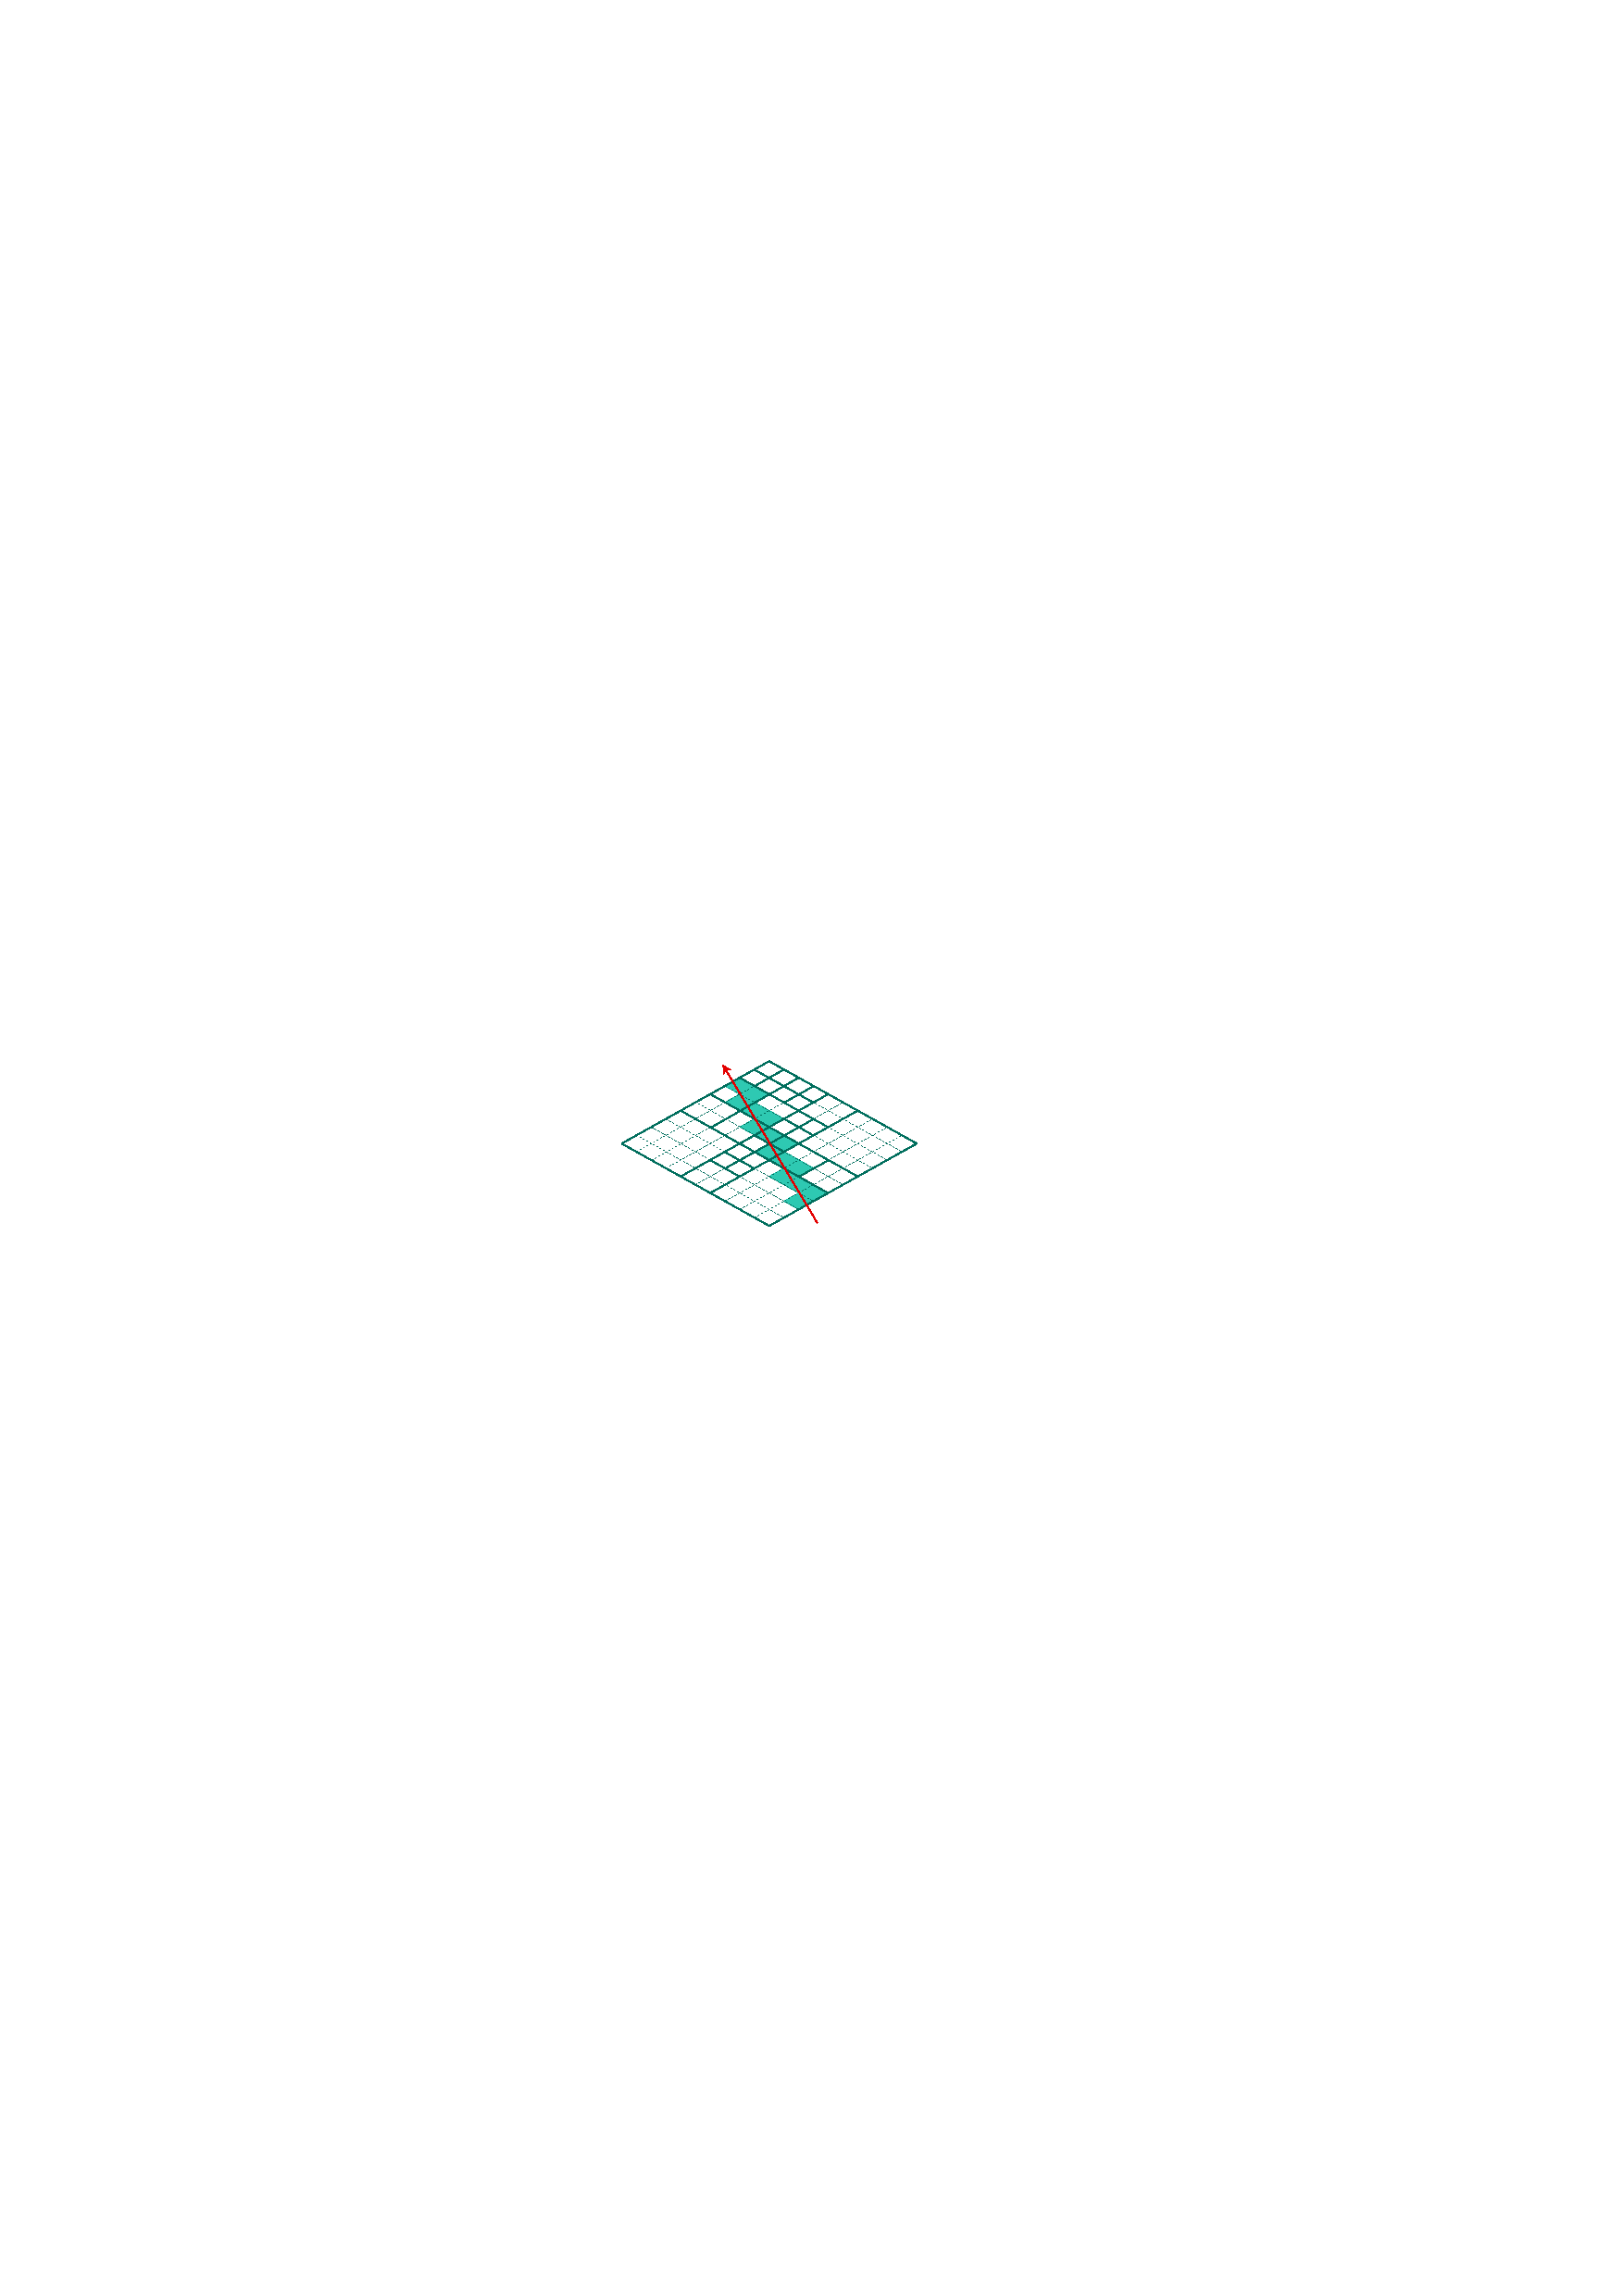
\includegraphics[scale=1]{figures/emptyspace_naive.pdf}
  \caption{Naive method visits all \newline logical voxels redundantly}
  \label{fig:emptyspace1}
\end{subfigure}%
\begin{subfigure}{.33\textwidth}
  \centering
  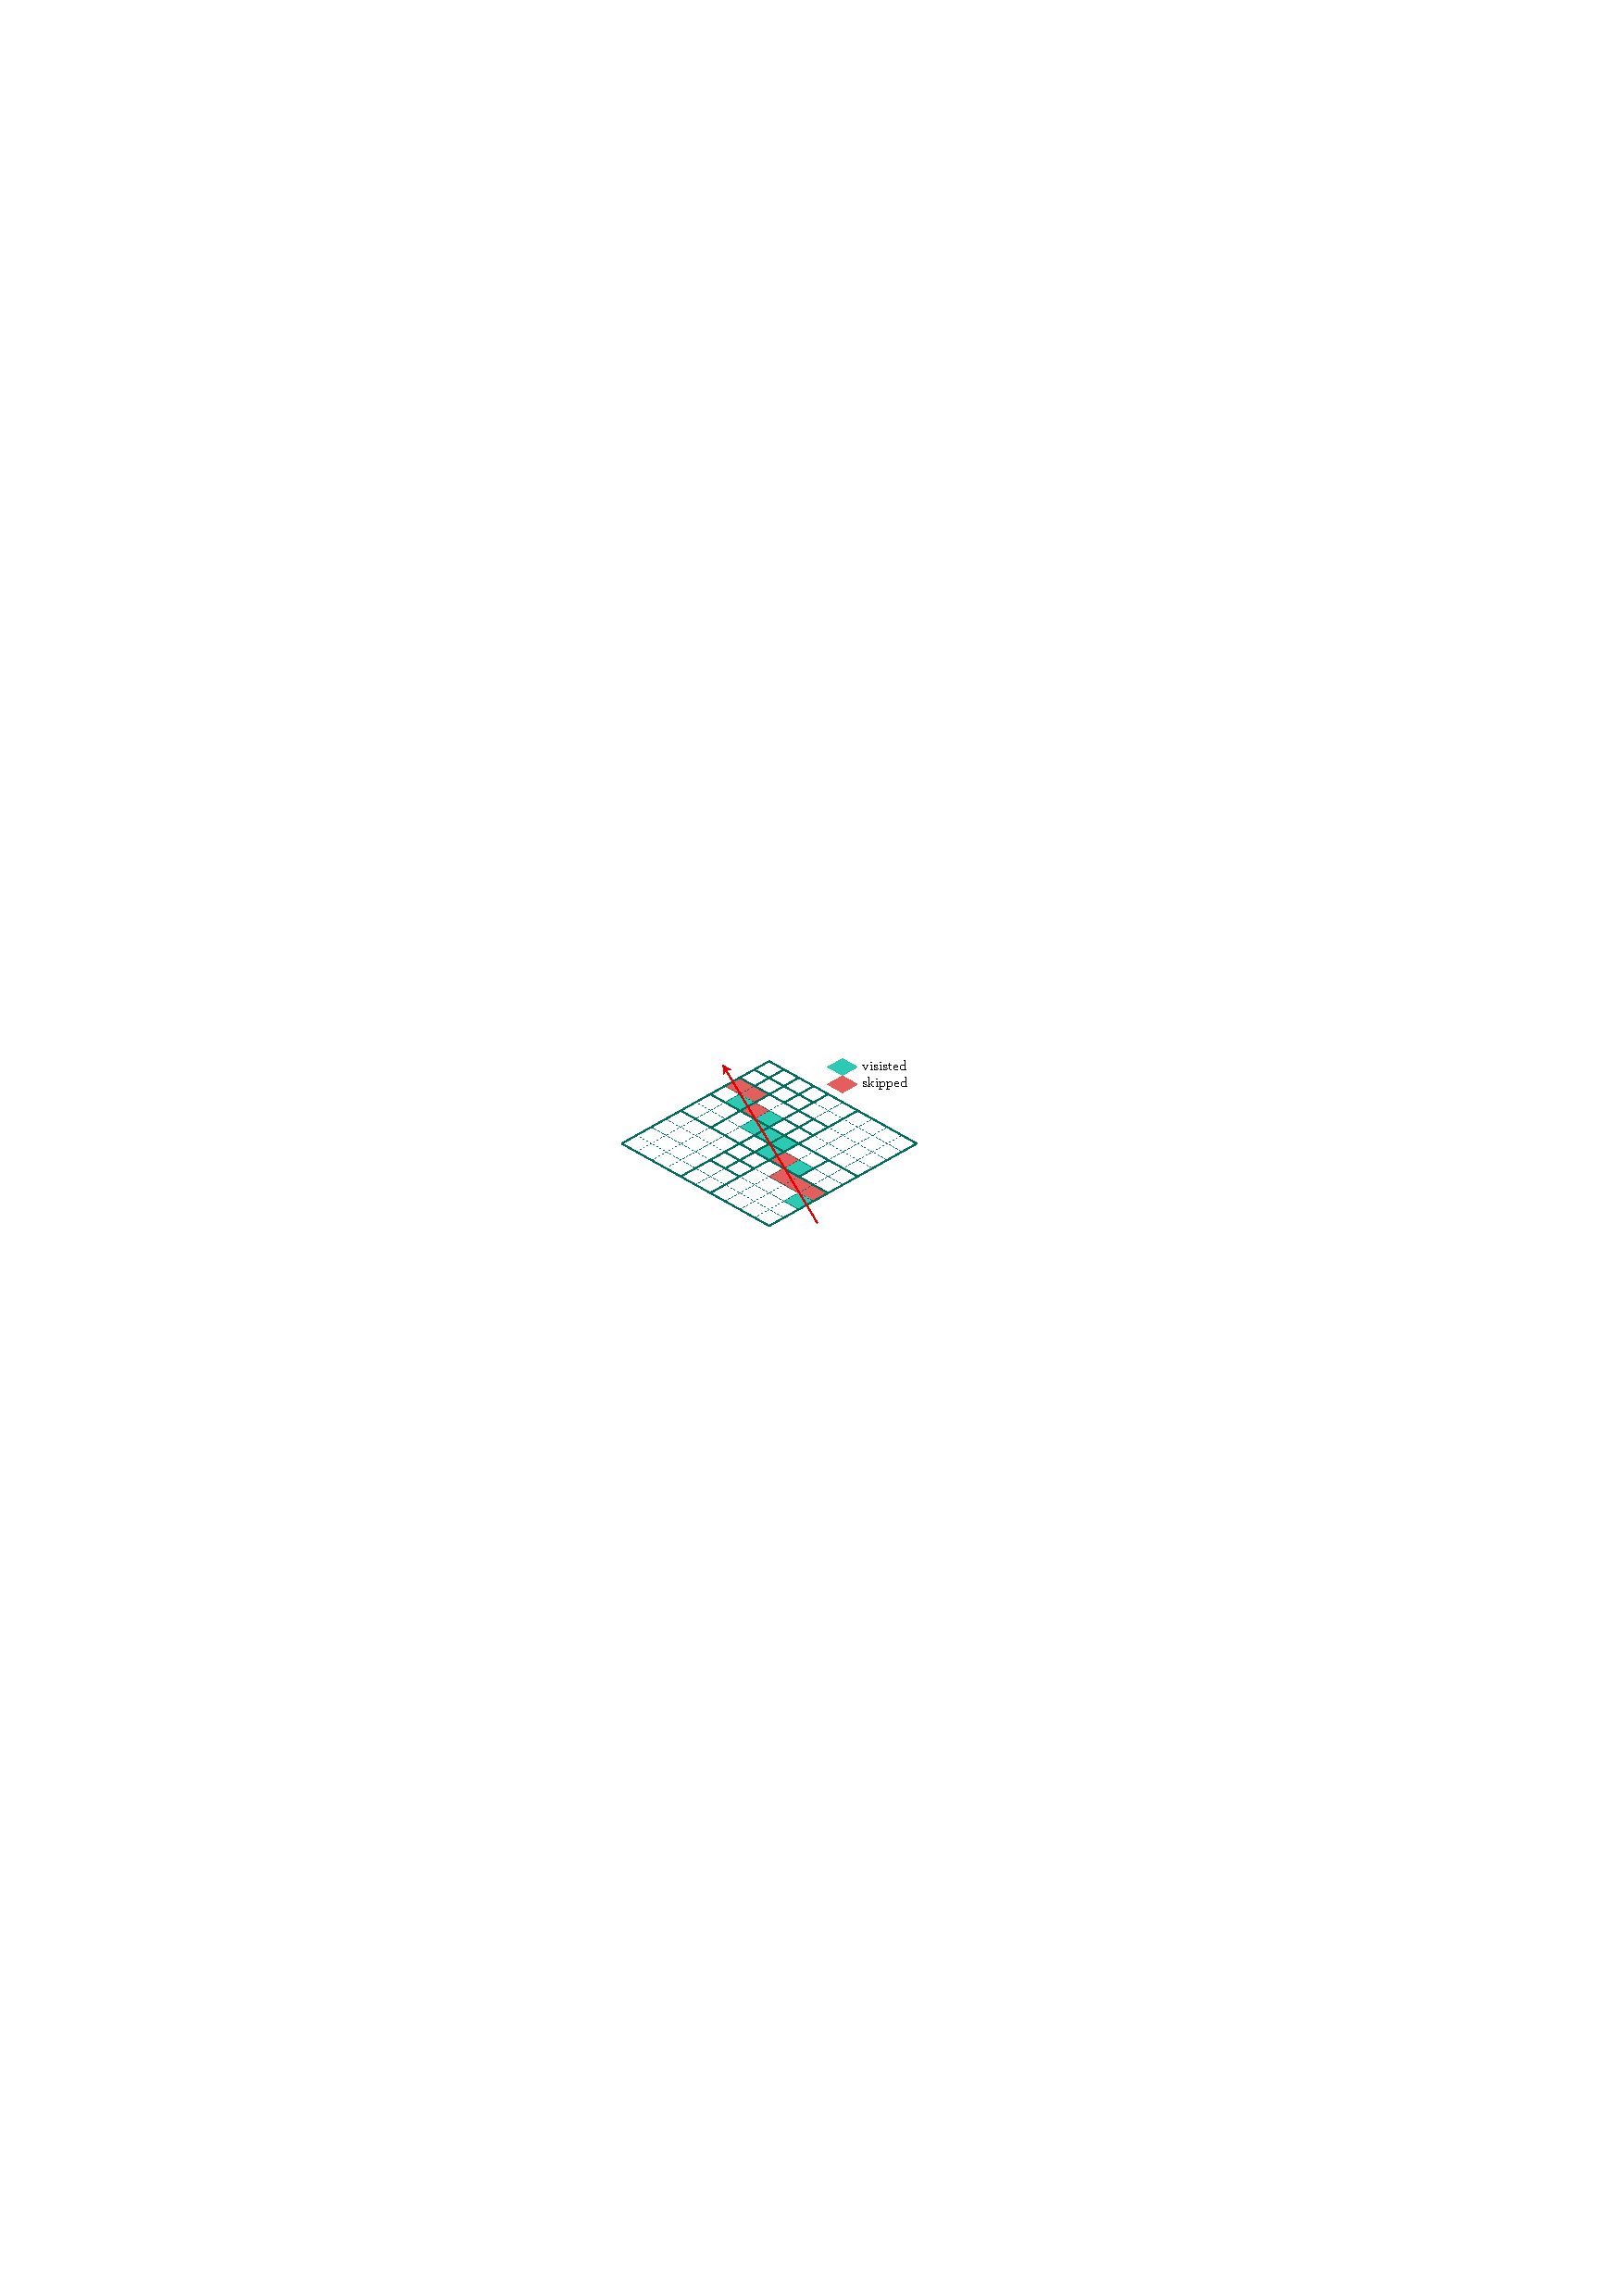
\includegraphics[scale=1]{figures/emptyspace_skip1.pdf}
  \caption{Making all steps, only visiting \newline relevant voxels}
  \label{fig:emptyspace2}
\end{subfigure}
\begin{subfigure}{.33\textwidth}
  \centering
  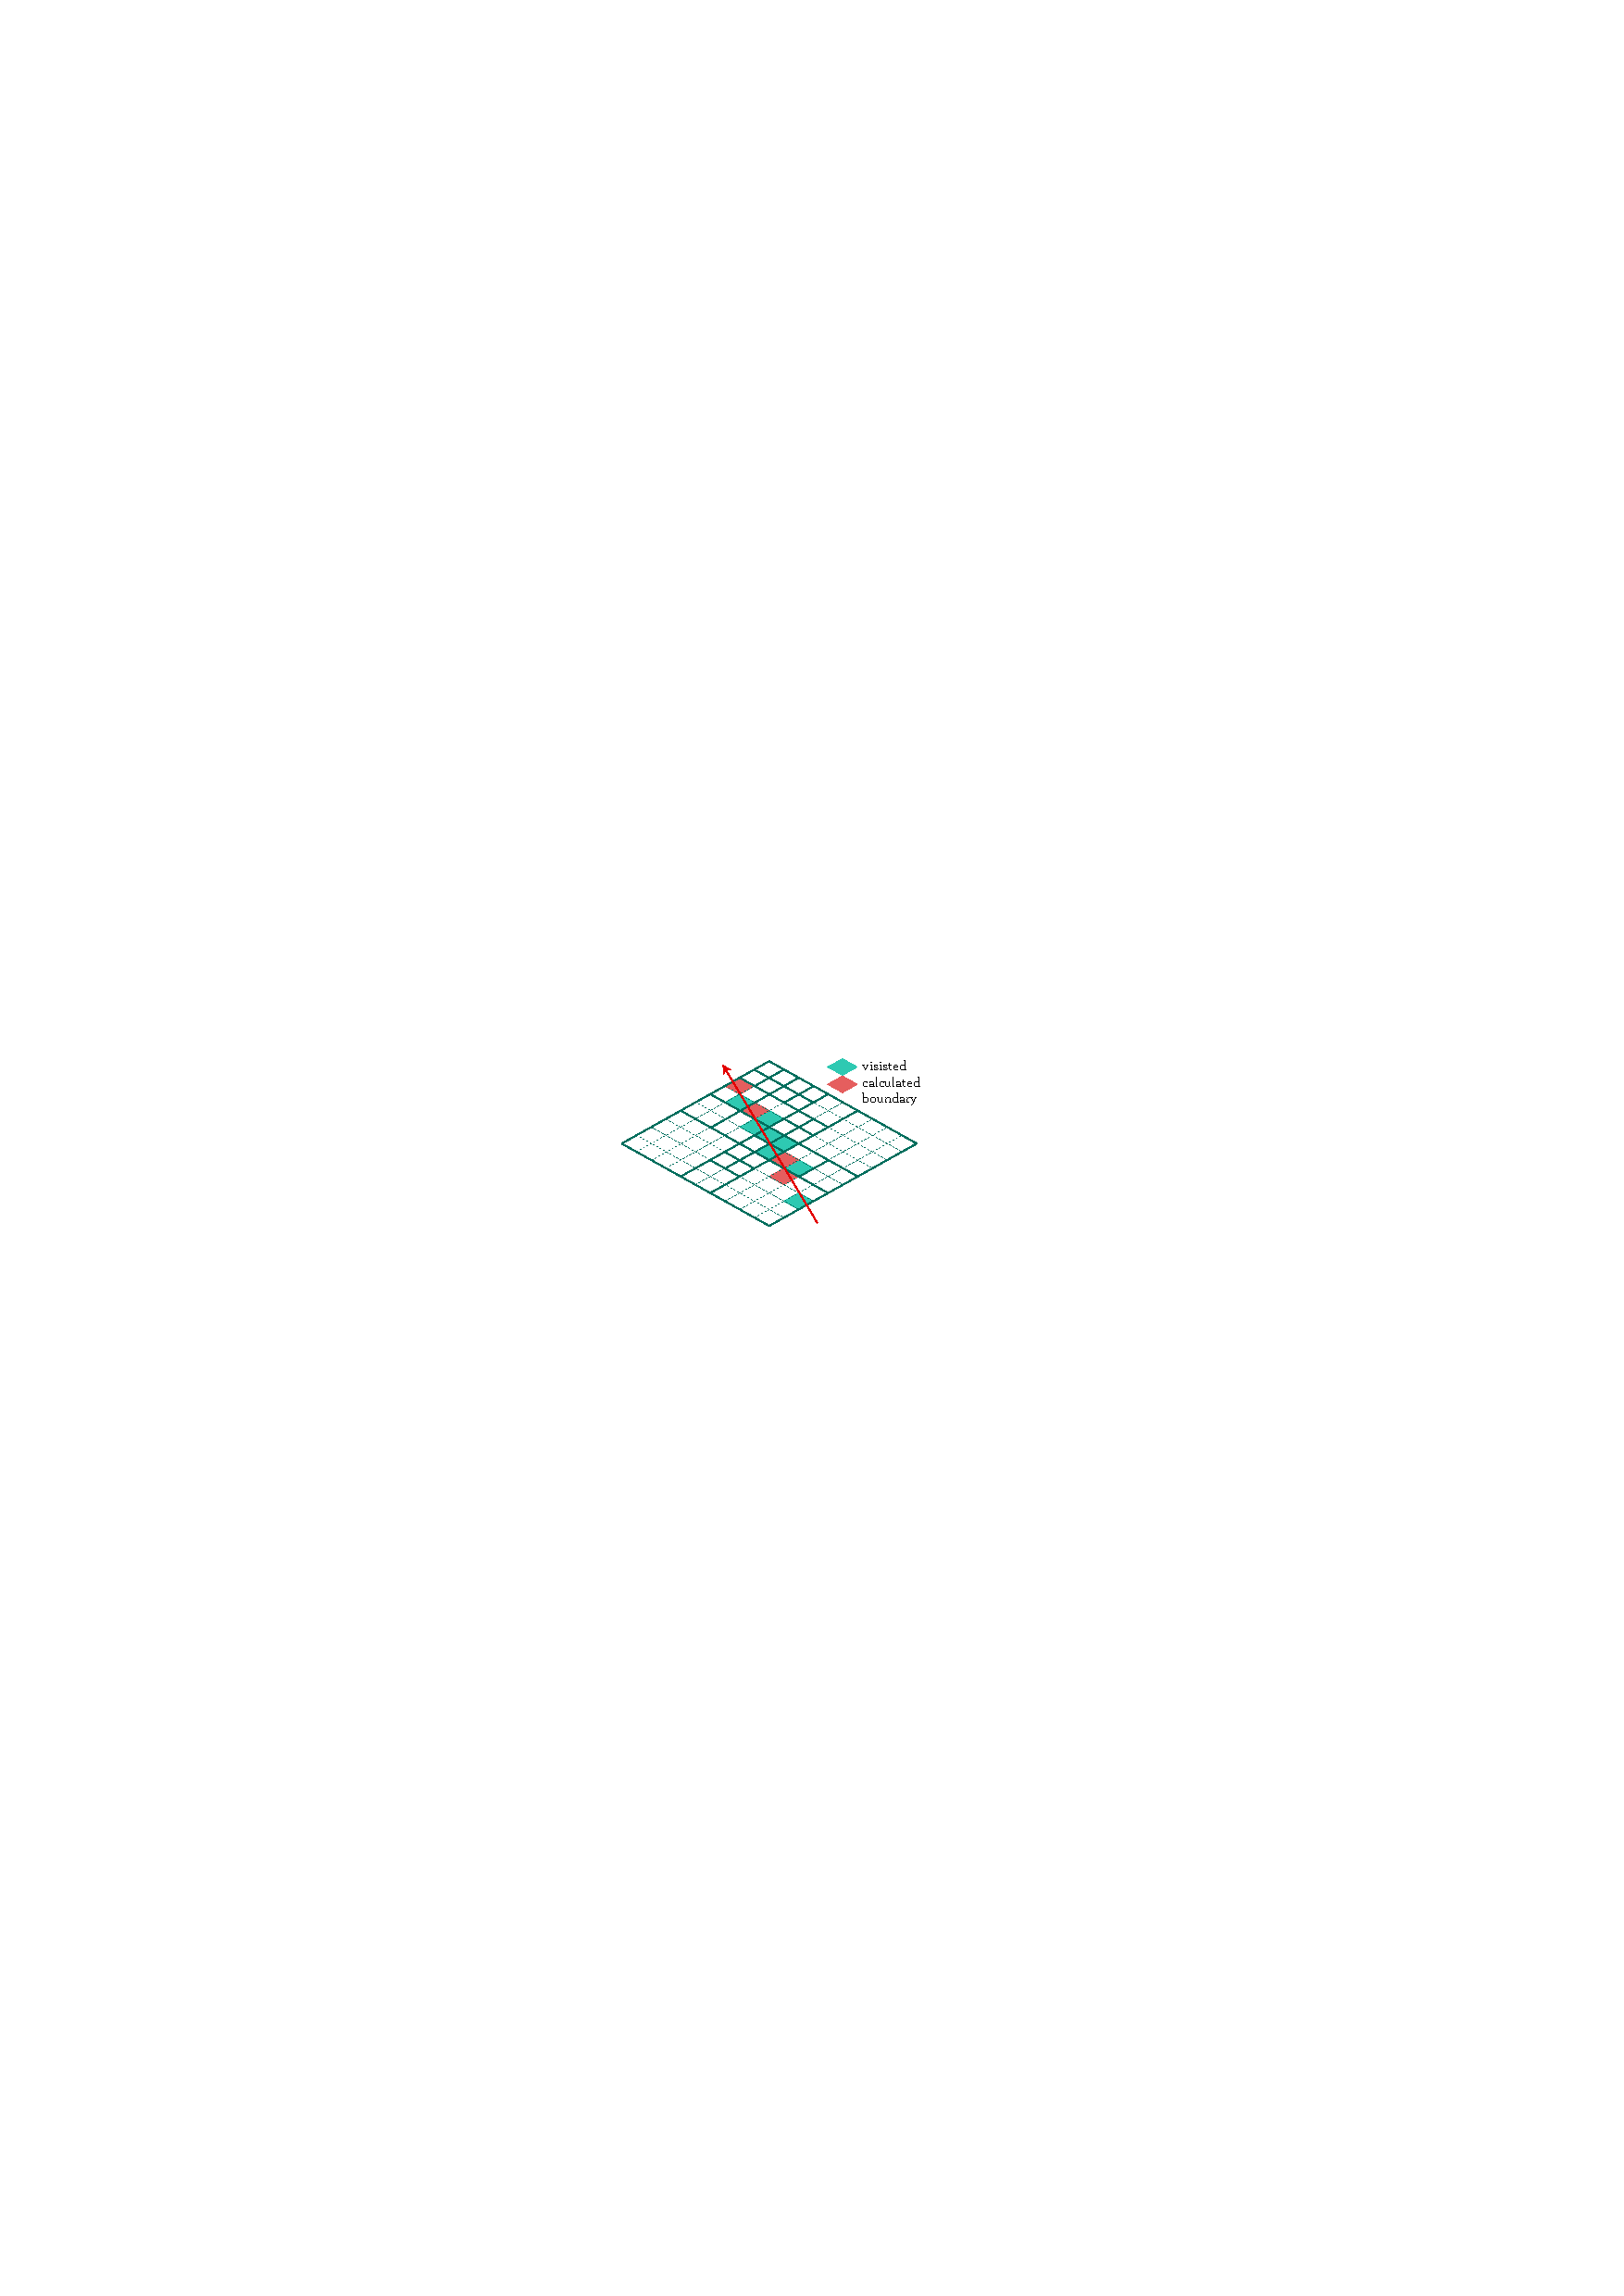
\includegraphics[scale=1]{figures/emptyspace_skip2.pdf}
  \caption{Calculating boundaries to do \newline  at most two steps per voxel}
  \label{fig:emtpyspace3}
\end{subfigure}
\caption{Different methods of skipping terminal blocks}
\label{fig:emptyspace}
\end{figure*}
The method mentioned in the last subsection, requires the algorithm to step through many logical voxels in order to finally reach its (useful) neighbour. Although no expensive instructions are required, it would be even better to have the ability to calculate the exact distance one has to travel to the neighbouring voxel. The problem is, however, that we can only perform a step at the smallest level (the logical voxelmap). So in the worst case, as many steps as a level's mipmap factor are required. 

In the work by Sung \cite{sung91} an algorithm is proposed that calculates the boundary to the neighbouring voxel, at an arbitrary level and in a constant amount of instructions. This means we can use one `complex step' as described by Sung (we are at the boundary then) and then one regular step to arrive at a neighbour. Figure \ref{fig:emtpyspace3} demonstrates this. While this is a very useful algorithm, our experiments demonstrated that the gain over the `obvious method' is generally small. This is partly due to the fact that it uses many additional registers on the GPU, and partly due to the fact that we already reduce the amount of mipmap levels significantly, so there was little gain to be had in the first place.
%
\subsection{Level-Of-Detail and Aliasing}
%
%
\begin{figure}[b!]
\centering
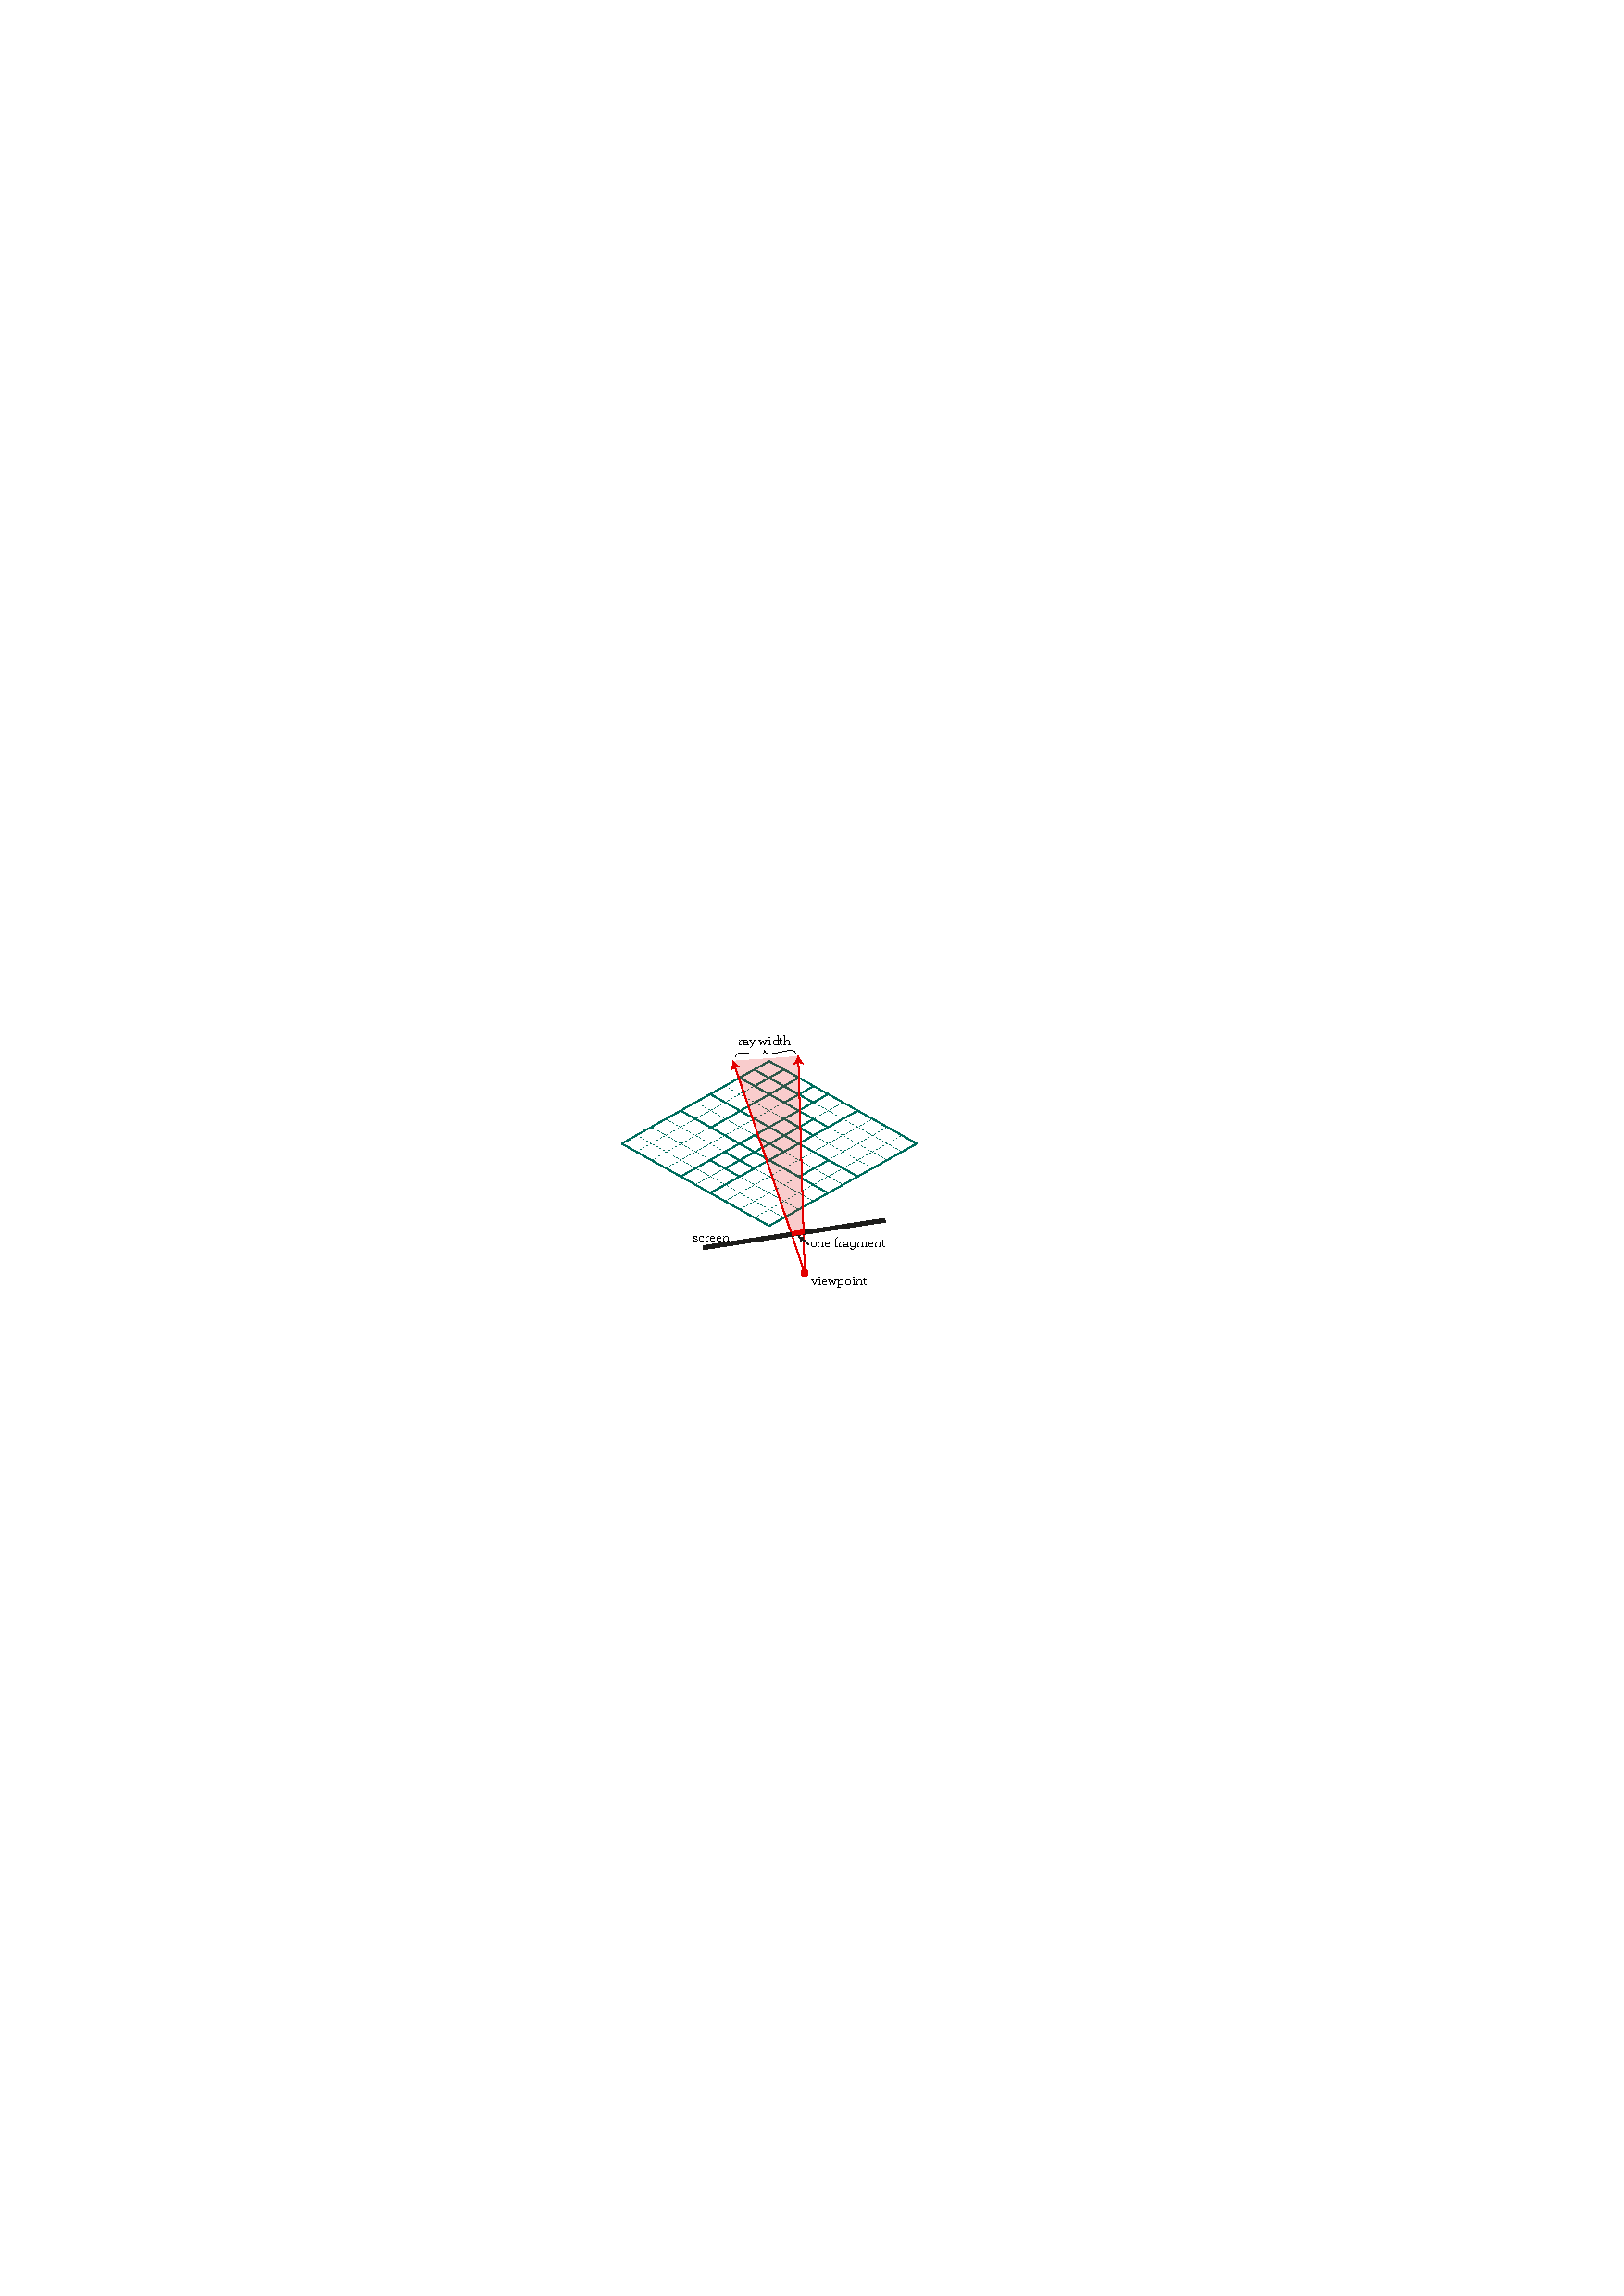
\includegraphics[scale=1.0]{figures/raytracing_cones.pdf} 
\caption{The ray-cone diverges as it progresses away from the camera}
\label{fig:cones}
\end{figure}
%
Sometimes it may not be necessary to refine until a terminal voxel is reached. Especially when the size of a fragment becomes larger than the size of an individual voxel, further refinement actually degrades the quality of the final image. In terms of signal processing it can be said than the detail of the geometry exceeds the Nyquist-frequency of the carrier (the screen). In this case aliasing of the signal will occur, resulting in unpleasingly looking edges in high-frequent details. Additionally, due to the grid structures of both the screen and the voxels, the \emph{moir\'e} phenomenon can occur. Moir\'e introduces false patterns where two grids of similar frequency are projected onto each other, also resulting in displeasing imagery.

The `perfect' solution to these problems is the \emph{oversampling} of the signal. In computer graphics, this is often called \emph{supersampling anti-aliasing} \cite{crow77} and basically means that for each fragment, multiple samples are taken and then averaged. So for each pixel, multiple rays need to be cast, resulting in significantly poorer performance.

The work by Amanatides \cite{amanatides84} demonstrates a much more elegant way that can be used with raytracing. Amanatides proposes that a ray is not a straight line, but should rather be modelled like a cone. As demonstrated by Figure \ref{fig:cones}, we are interested in the integral of the cone instead of a singular sample hit by an infinitely thin line. By using a cone with the correct `divergence', depending on the resultion and field-of-view, the resulting image is free of aliasing and moir\'e. While this technique is costy in raytracing, it is rather simple in discrete raycasting, given a the volume is in a \emph{level-of-detail} (LOD) structure.
%
In a level-of-detail structure (MIP maps and SVOs are examples of such structures), a filtered sample is availabe for every level of detail of the original image. So if the ray hits the volume near the camera, a completely refined voxel is taken, while far from the camera a less or unrefined voxel is used. Since every sample is a filtered average of lower levels, we instantly obtain the integral of the cone. Apart from being beneficial for the image quality, we gain in performance as the depth traversal may be terminated earlier.

An SVMM encoded voxelmap is only an LOD structure if $w=2$, which will almost never be the case. Due to this fact, the principle of filtering using LOD can only be partly achieved. It can still improve image quality and performance, but we also believe that anti-aliasing should be implemented as a post-processing step. This post-processing can be done using, for example, a bilateral filter \cite{eisemann04}. Using such a filter is a relatively small performance penalty, while it also can improve quality of object-background and object-object edges as well as the smoothing of ambient occlusion and normals - all of which the cones technique cannot.
%
\subsection{Precision}
The baseline algorithm uses incremental arithmetic on single-precision floating point numbers. On really large volumes this approach may eventually lead to artifacts. The work of Stolte et al. \cite{stolte95} proposed a method to alleviate this problem, although it was not designed for modern graphics hardware. Using anything other than floating points will severely degrade the performance on modern GPUs (some support double precision, but at half the speed). In our experiments, these artefacts were generally acceptable and almost removed by post-render anti-aliasing. Nevertheless, it is a cause for concern. One could also lower the precision further by changing lines 13-14 to use $\lfloor t_{max} \rfloor$. The algorithm may now pick multiple axes to traverse, making the traversal some 30\% faster. See Figure \ref{fig:precision}. This optimization does however introduce noticeable artefacts.

\begin{figure*}
\centering
\begin{subfigure}{.33\textwidth}
  \centering
  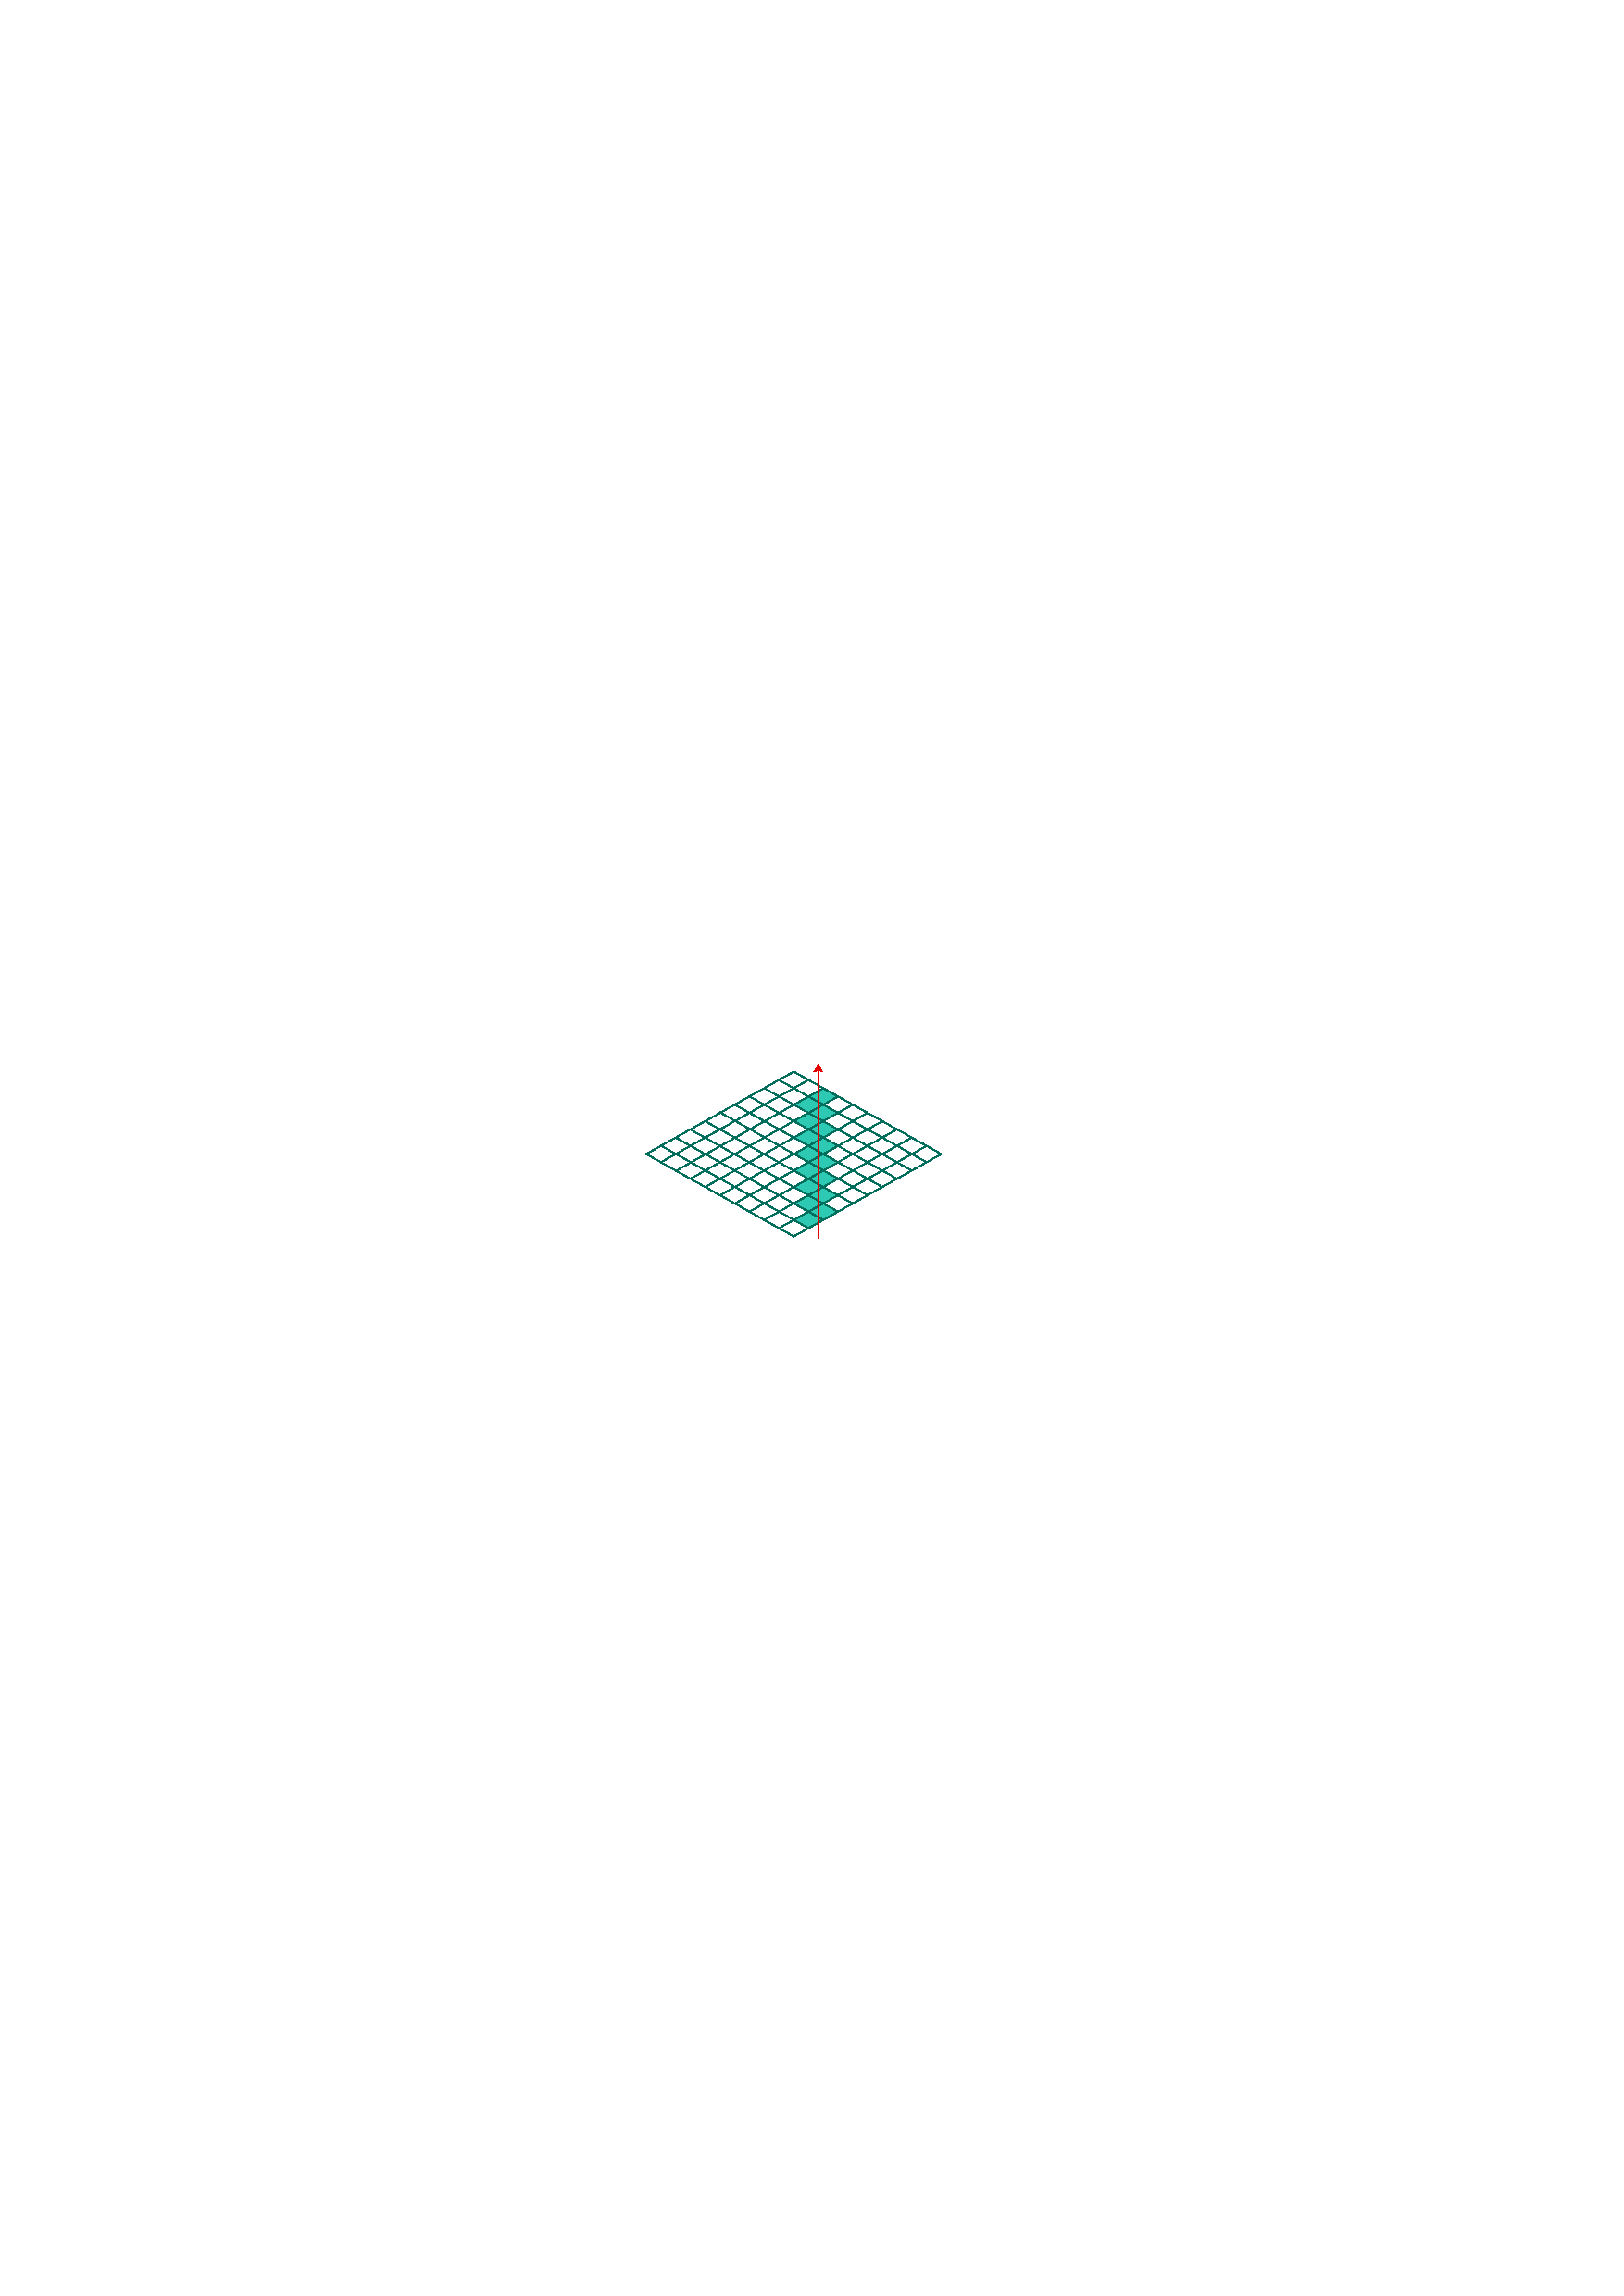
\includegraphics[scale=1]{figures/dda_precise.pdf}
  \caption{Travelling one axis at a time}
  \label{fig:precision1}
\end{subfigure}%
\begin{subfigure}{.33\textwidth}
  \centering
  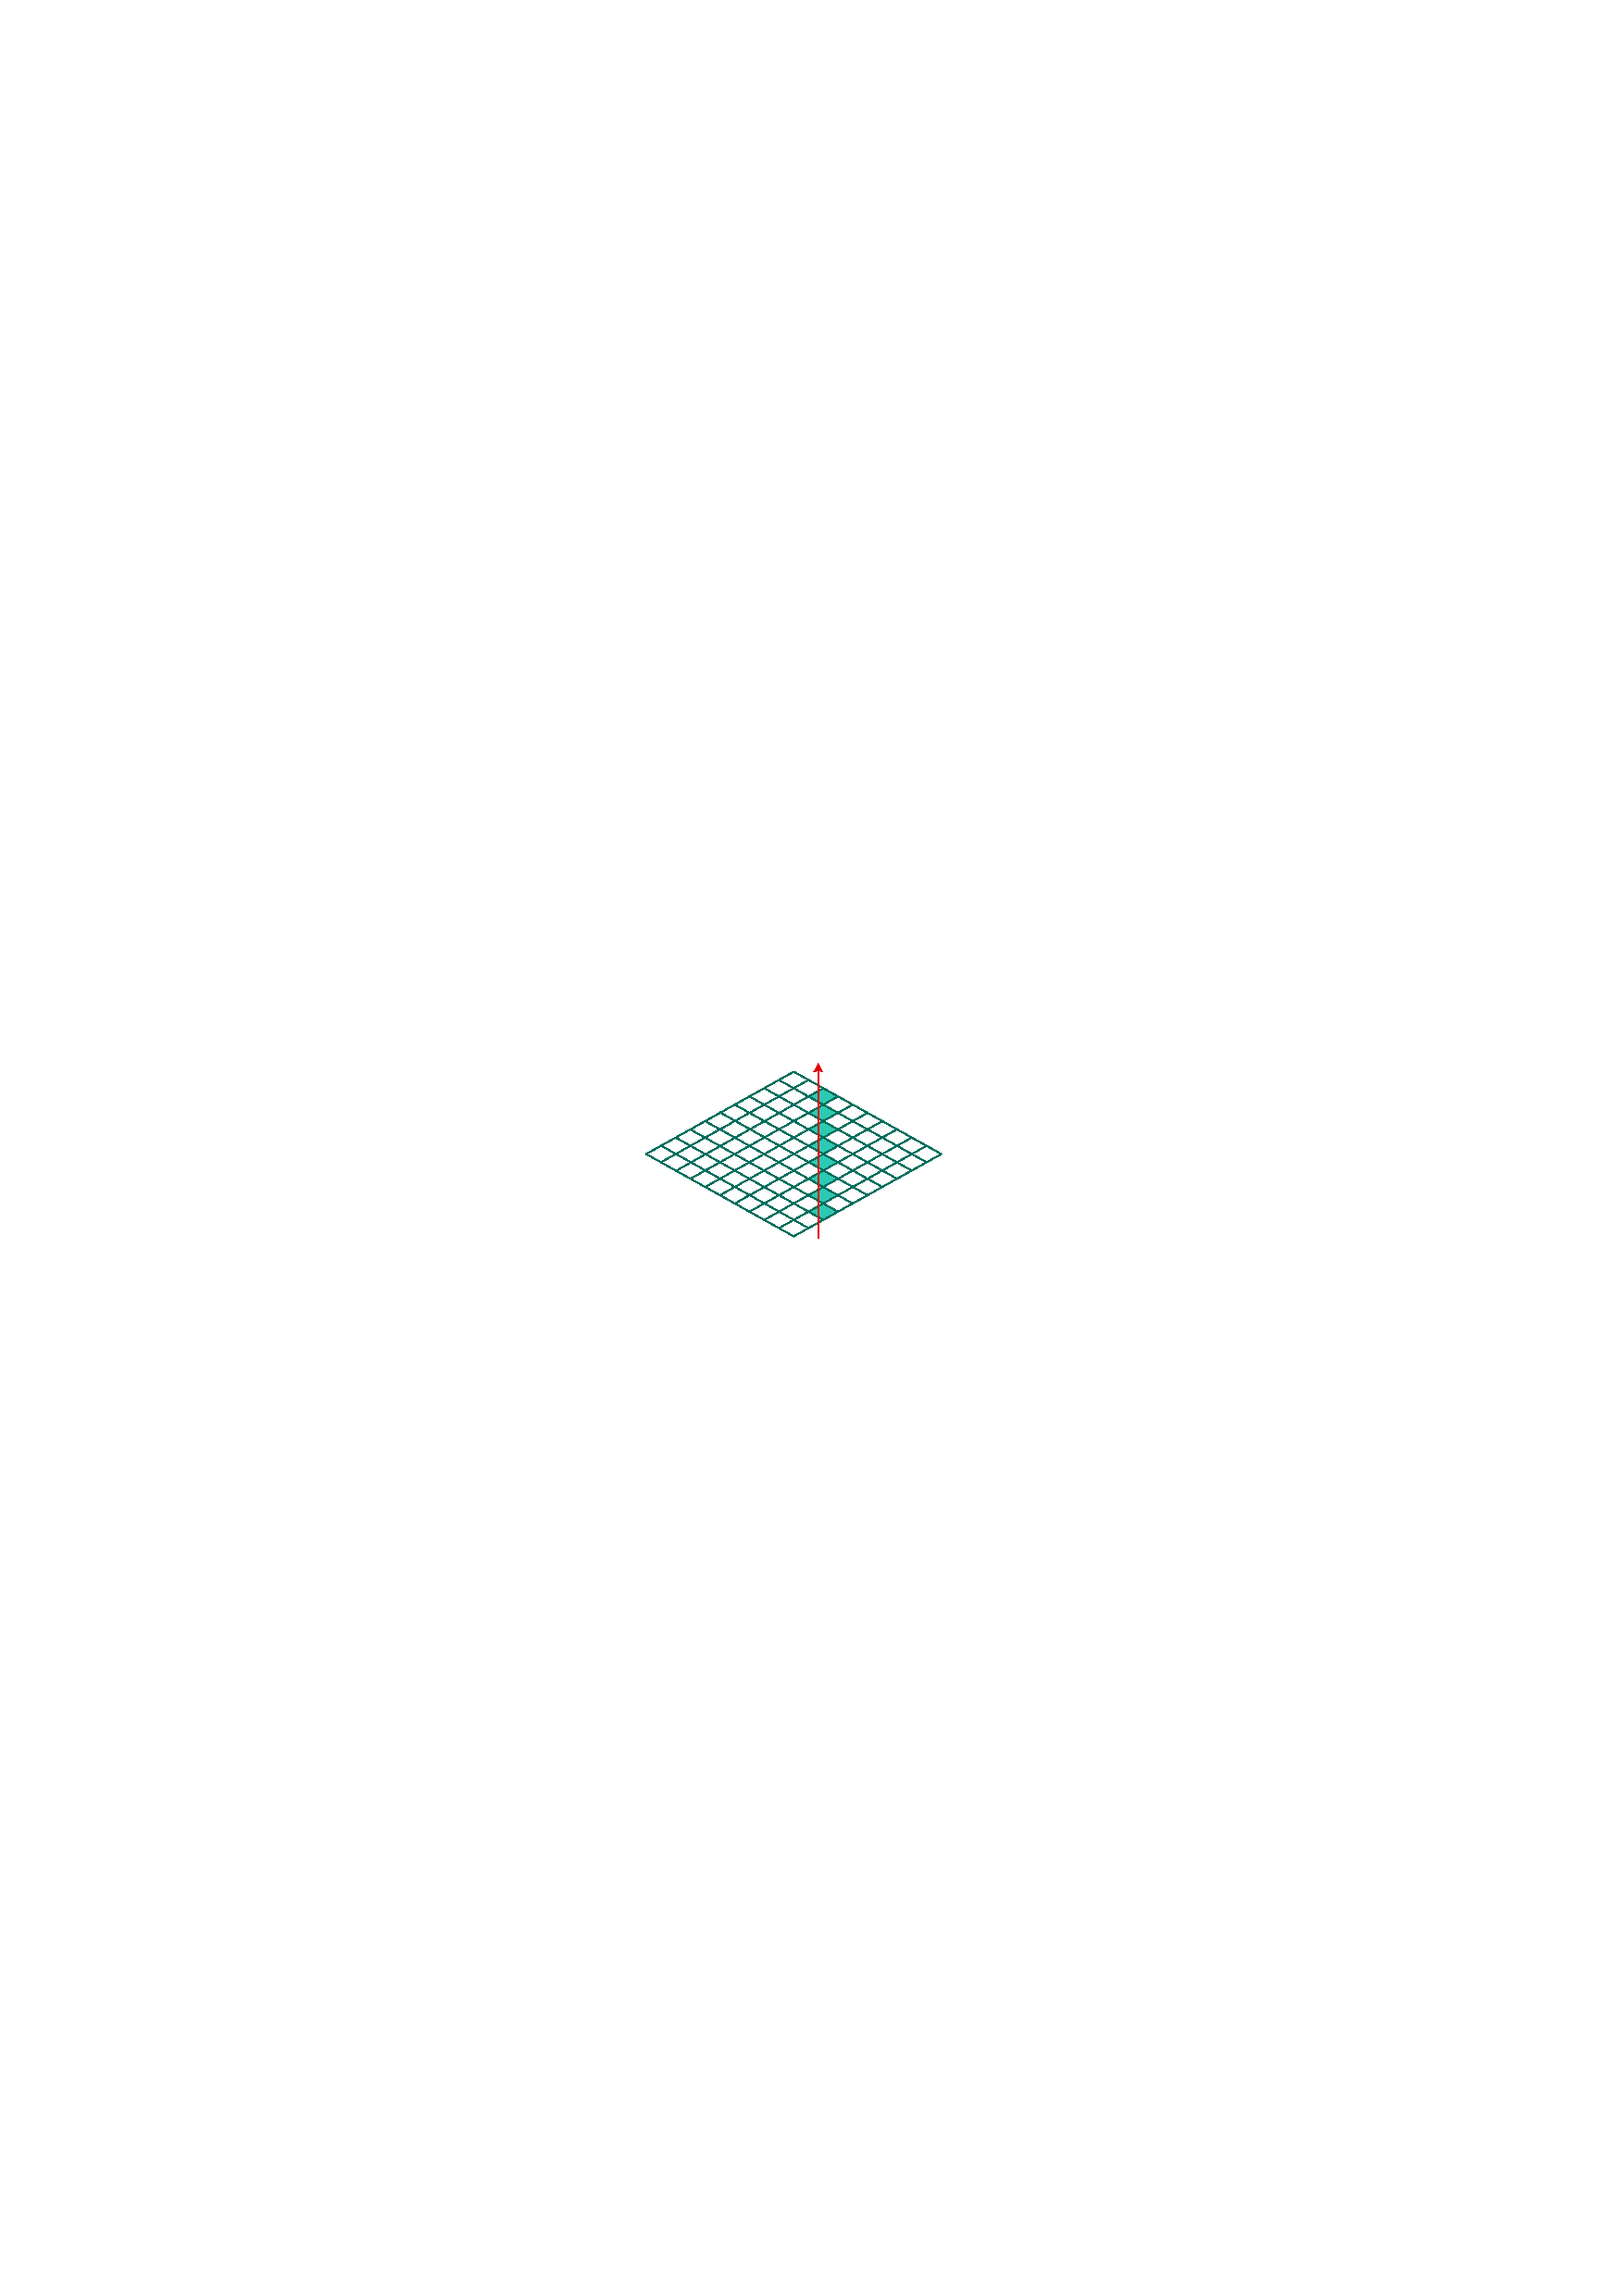
\includegraphics[scale=1]{figures/dda_imprecise.pdf}
  \caption{Travelling multiple axes at a time}
  \label{fig:precision2}
\end{subfigure}
\begin{subfigure}{.33\textwidth}
  \centering
  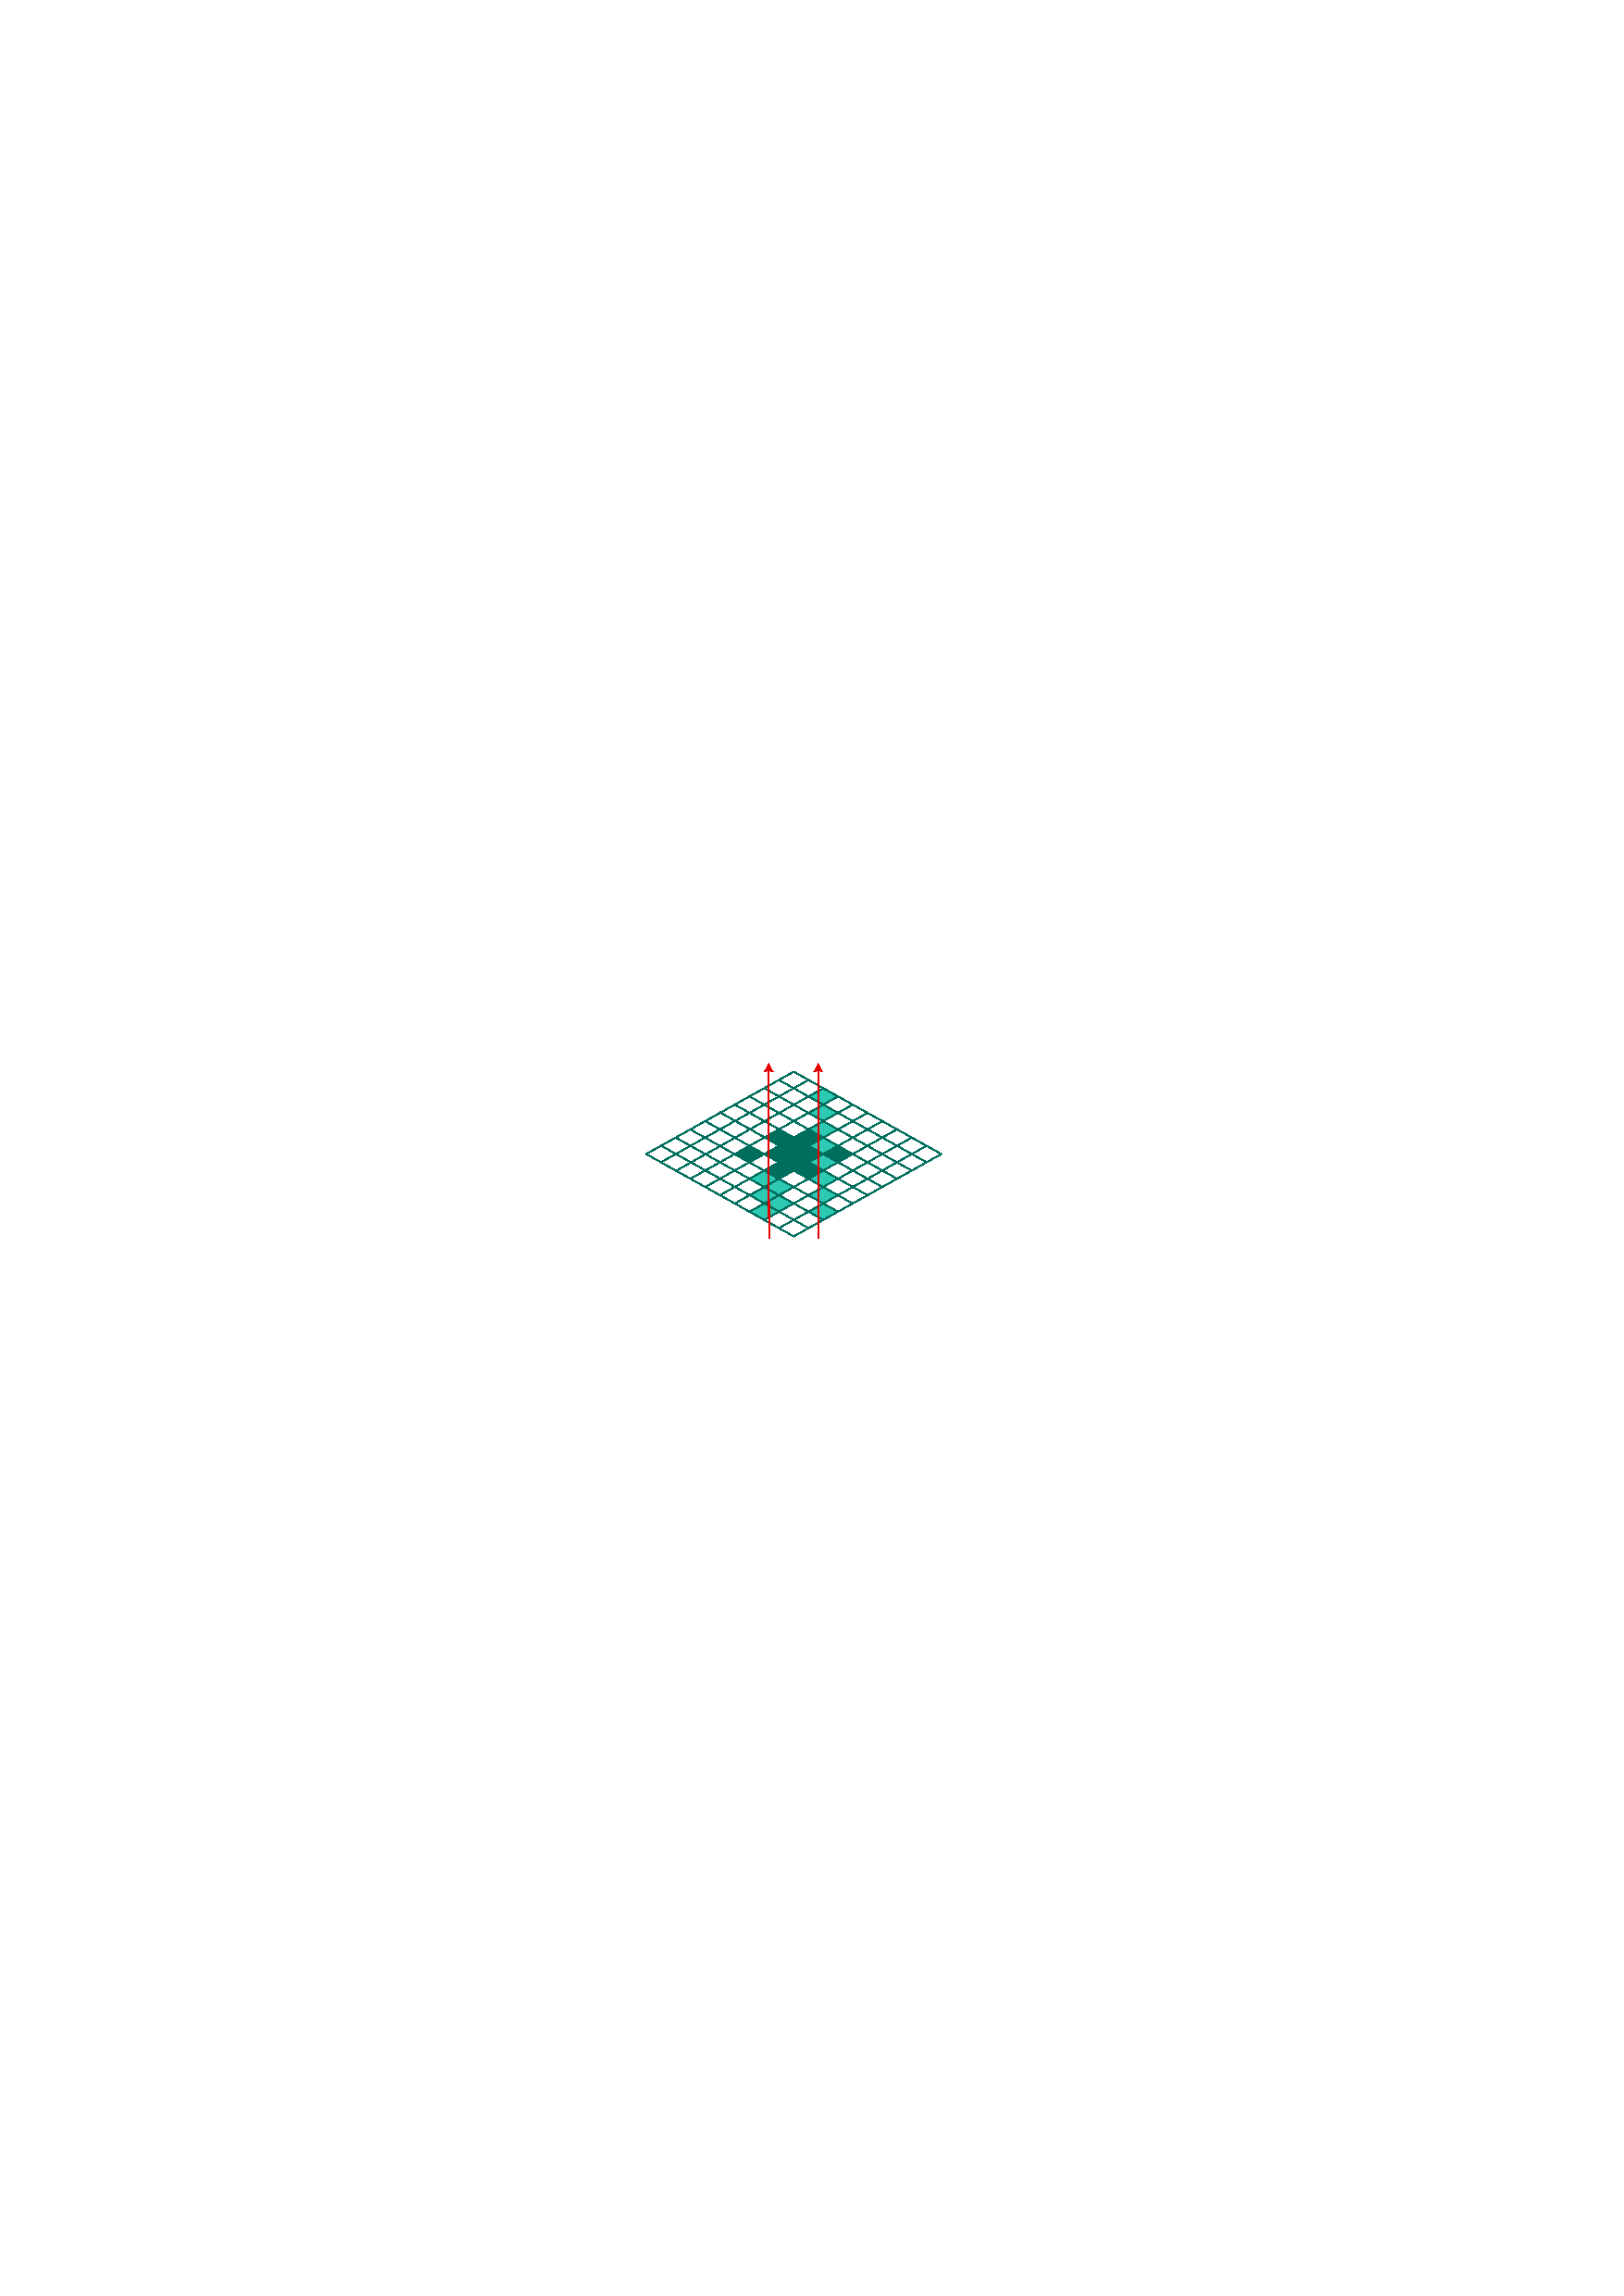
\includegraphics[scale=1]{figures/dda_miss-hit.pdf}
  \caption{Imprecise traversal (right) compared to more precise traversal (left)}
  \label{fig:precision3}
\end{subfigure}
\caption{Travelling multiple axes at a time can save up to 66\% visits, but imprecise traversal may miss fragile geometry.}
\label{fig:precision}
\end{figure*}
%
\section{Block memory management}
%
The linear structure that the SVMM encoder uses to write individual blocks to the disk, cannot be used to store the data on the GPU. We can, however, exploit the 3D texture features of the hardware. By allocating a large enough 3D texture to form a \emph{block pool}, it is possible to store all blocks from one level in their original order and still benefit from the spatial caching. In order to do this, one block pool per mipmap level is created. Because different levels can have a different block width, it would be impractical to store all those differently sized blocks in a 3D structure. Secondly, a hash function is needed to translate the offset of a block to a set of texture coordinates. 

Before a hash function can be created, the optimal size $(U,V,W)$ of the pool must be established, given an amount of blocks $N$.
\begin{align*}
c &= \lfloor \sqrt[3]{N} \rfloor\\
U = V &= 2^{\lfloor \log_2{c} \rfloor} &\text{Round $c$ to the nearest power of two}\\
W &= \lceil \frac{N}{U*V} \rceil &\text{The remaining space is allocated in the W-direction}
\end{align*}
By making $U$ and $V$ a power of two, the hash function can make use of arithmetic shifts instead of divisions. The waste of space that is inherent to the rounding is, when empirically tested, quite small for even billions of blocks.

Now a hash function $\mathbf{H}(o)$ can be defined that translates a block offset $o$ within a certain level, to texture coordinates $(u,v,w)$. 
\begin{align*}
\mathbf{H}(o) &= \begin{dcases} 
    u = o - (v + w) = o - \Big\lfloor \frac{o - \lfloor \frac{o}{UV} \rfloor }{V} \Big\rfloor - \Big\lfloor \frac{o}{UV} \Big\rfloor\\
    v = \Big\lfloor \frac{o-w}{V}  \Big\rfloor = \Big\lfloor \frac{o - \lfloor \frac{o}{UV} \rfloor }{V}  \Big\rfloor \\
    w = \Big\lfloor \frac{o}{UV} \Big\rfloor
\end{dcases}
\end{align*}
The practical implementation of this function is very fast by means of incremental arithmetic and shift operations.
%
\section{The rendering pipeline}
%
The \emph{geometry phase}, such as discrete raycasting in this case, is often part of a larger rendering pipeline. The raycasting as described in this chapter only deals with the color of a fragment based on its geometry (volume). Other steps may, for example, deal with reflections, lighting, refraction and anti-aliasing. Nowadays, it is increasingly common to implement these steps in \emph{screen space}, which means that they are performed after the geometry phase on a per-fragment basis (sometimes also called \emph{deferred rendering}). The advantage is that the complexity is given by the screen resolution and not by the resolution of the geometry, while the main disadvantage is that it is often an approximation of lesser quality. Often some additional data is required to enable screen-space calculations, such as the fragment's depth, normals or world position calculated during the geometry phase. 

The implementation that is used for the evaluation of our work, uses a set of simple screen space rendering steps. Lighting can either be provided by a simple Phong-Blinn shader or screen space \emph{ambient occlusion} (SSAO, see \cite{ssao}). In addition to the LOD-based anti-aliasing provided by the MIP mapping, a very simple depth-based anti-aliasing is performed. To make any of these steps possible, however, fragment normals need to be approximated first.
%
\subsection{Screen-space normal approximation}
%
While outside the scope of this thesis, we feel the necessity to briefly discuss the problems we encountered related to normals in a (discrete) volumetric data set. The term \emph{normal} refers to a vector that is perpendicular to a certain surface, while also being of unit length and pointing `out of the surface'. Normals are one of the basic building blocks in computer graphics and are used for almost any imaginable computation of 3D surfaces.  In reality, a voxelized surface can only have normals pointing in the directions of the six faces of a cube. This results in a low image quality and unnatural lighting. Therefore, if we assume that the surface represented by the voxels is smooth, we can try to approximate this surface and calculate its normals.

An approach that works on continuous geometry, is to calculate each fragment's position from the depth buffer and then calculate its normal using the positions of its neighbouring fragments. Voxelized geometry is, however, inherently discrete and the depthbuffer is therefore discontinuous. See also Figure \ref{fig:normals-depth}. The depth buffer can be smoothed to a certain degree, by using the linear filtering mode of the hardware texture units. For every texel that is requested, the surrounding texels are also obtained and interpolated. 

By using the interpolated depth, we can calculate the world-space positions of the surrounding fragments. We then use a circular sample pattern and construct triangles from the original fragment to the points on the circle. We repeat this while increasing the radii of the circles until (approximately) the size of a voxel is covered. We also check the depth of the samples agains the original fragment. If the difference is beyond some treshold, the sample is rejected in order to respect the occlusion boundaries. Figure \ref{fig:normals-approx} further demonstrates this principle.

For a complete survey of some more sophisticated methods, we refer the reader to \cite{yagel92}.

\begin{figure*}[b]
\centering
\begin{subfigure}{.4\textwidth}
  \centering
  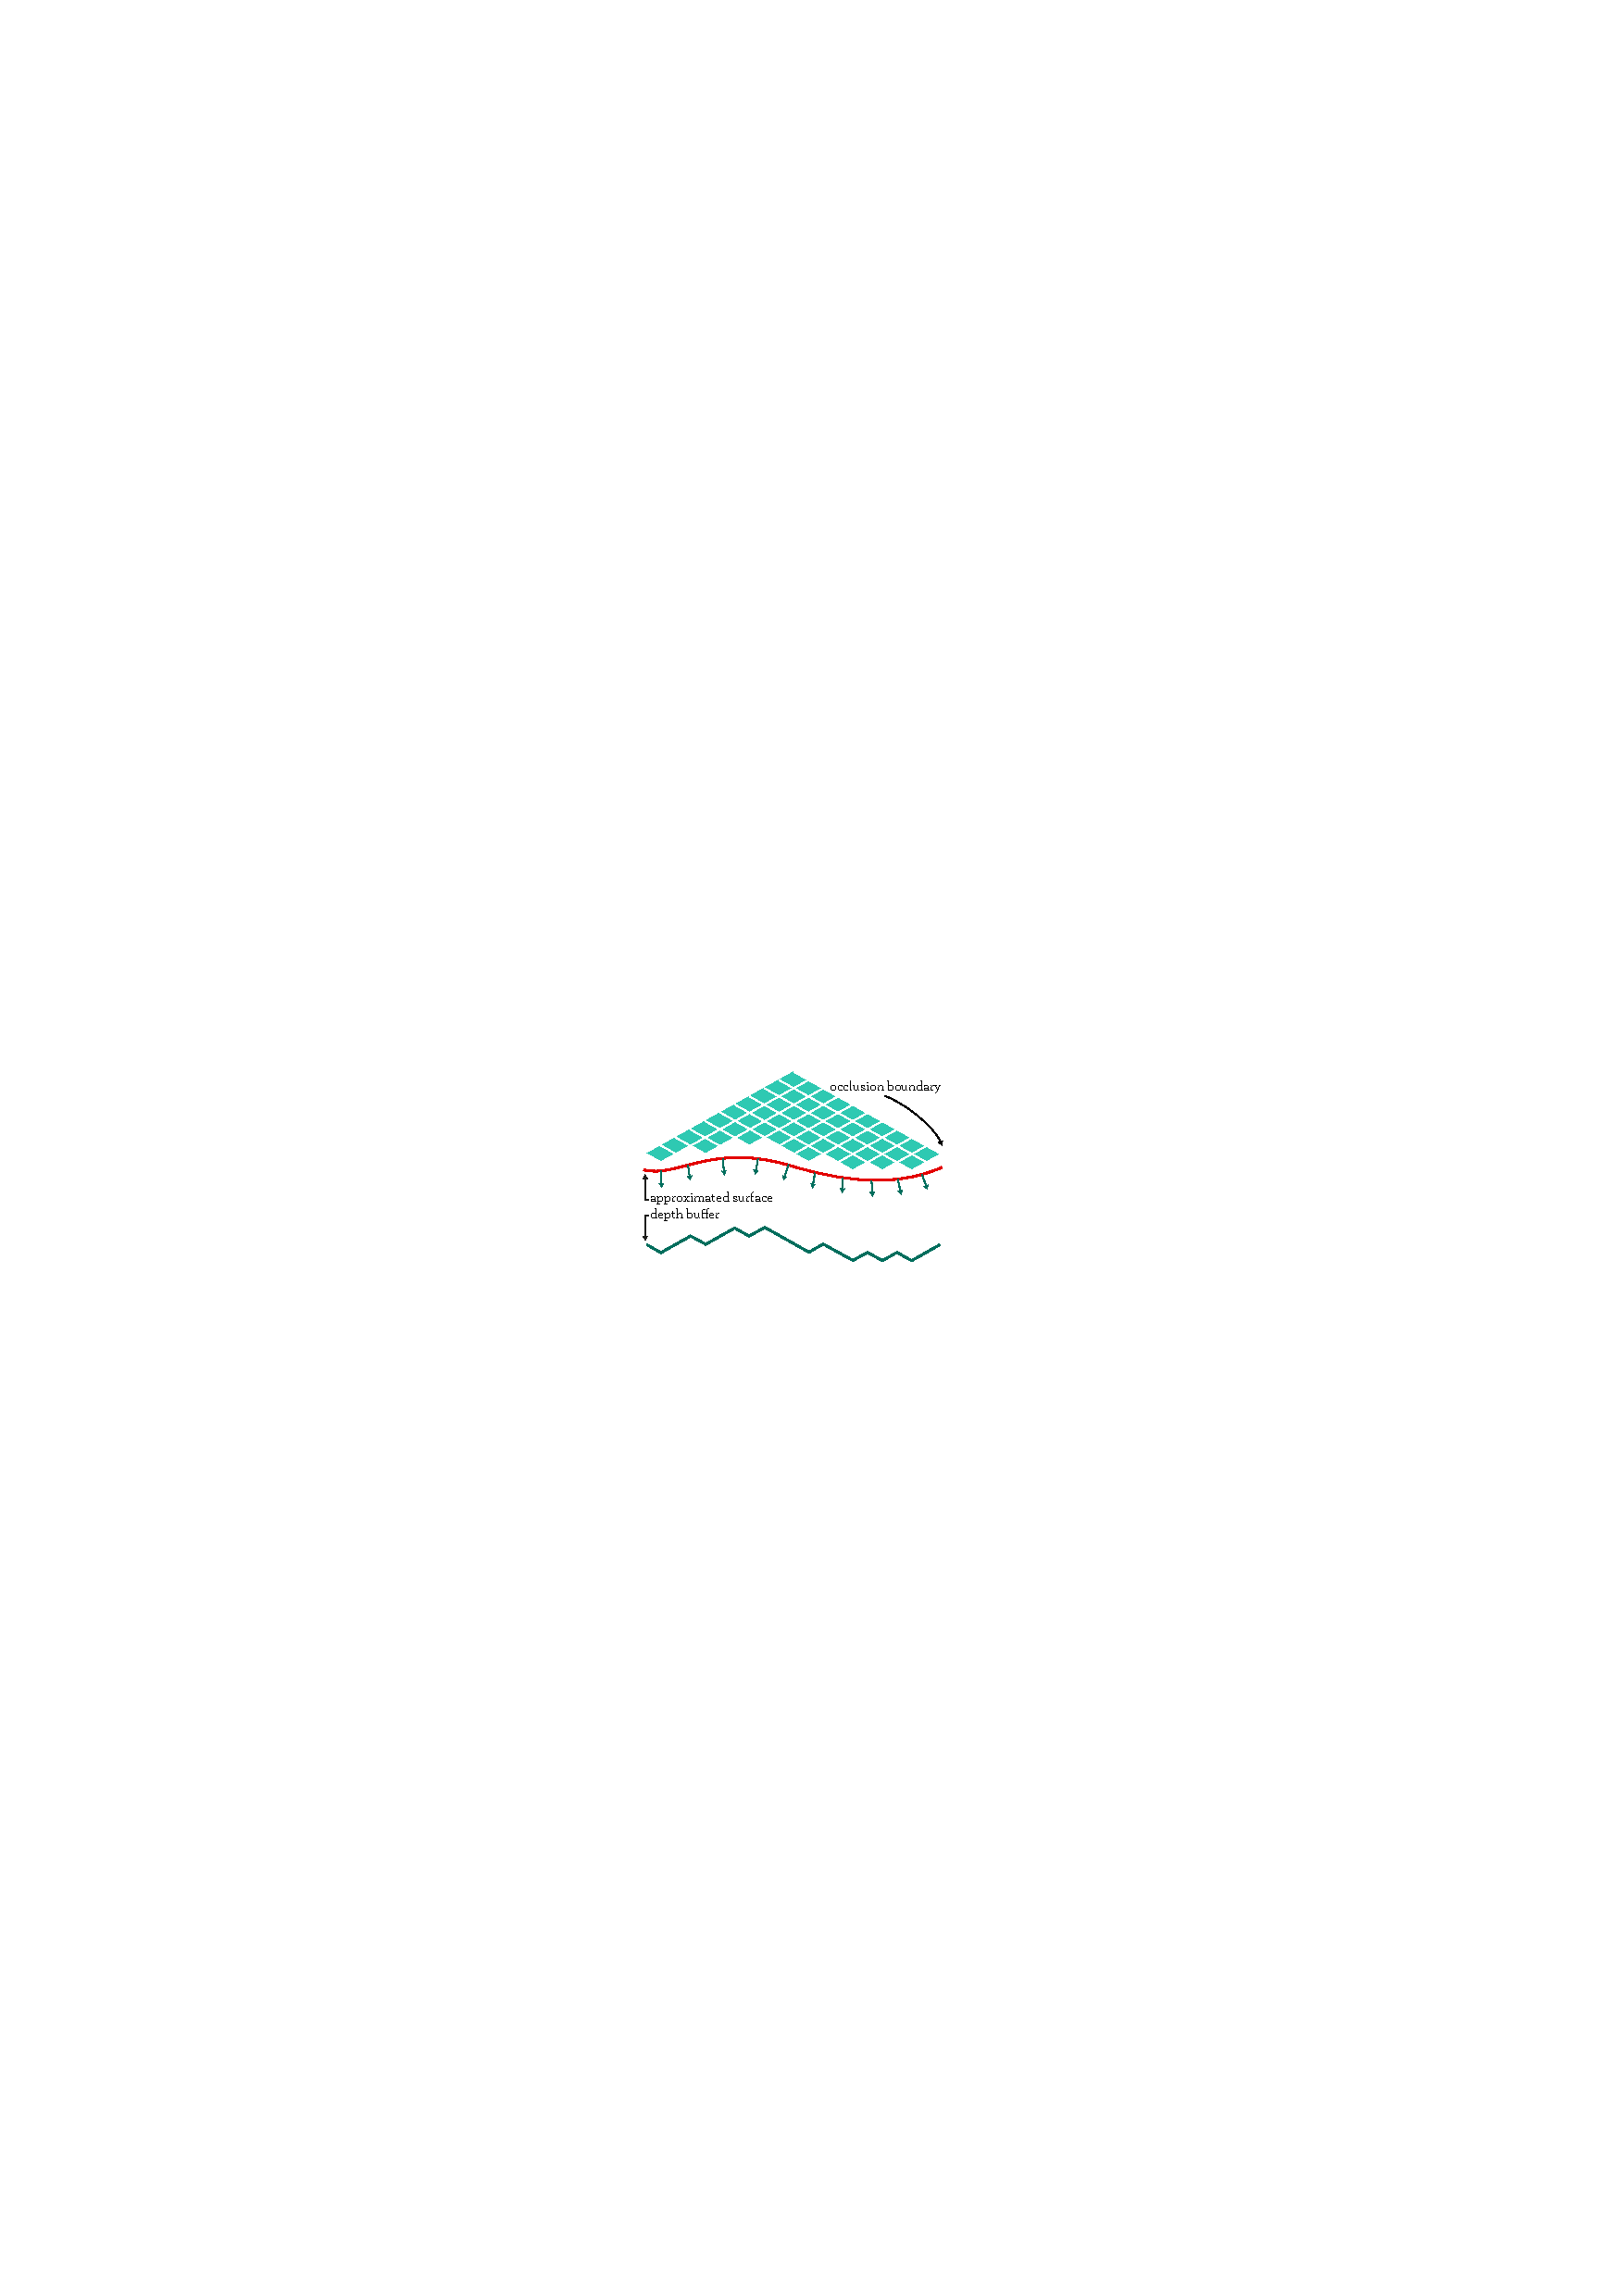
\includegraphics[scale=1.2]{figures/normals.pdf}
  \caption{}
  \label{fig:normals-depth}
\end{subfigure}%
\begin{subfigure}{.6\textwidth}
  \centering
  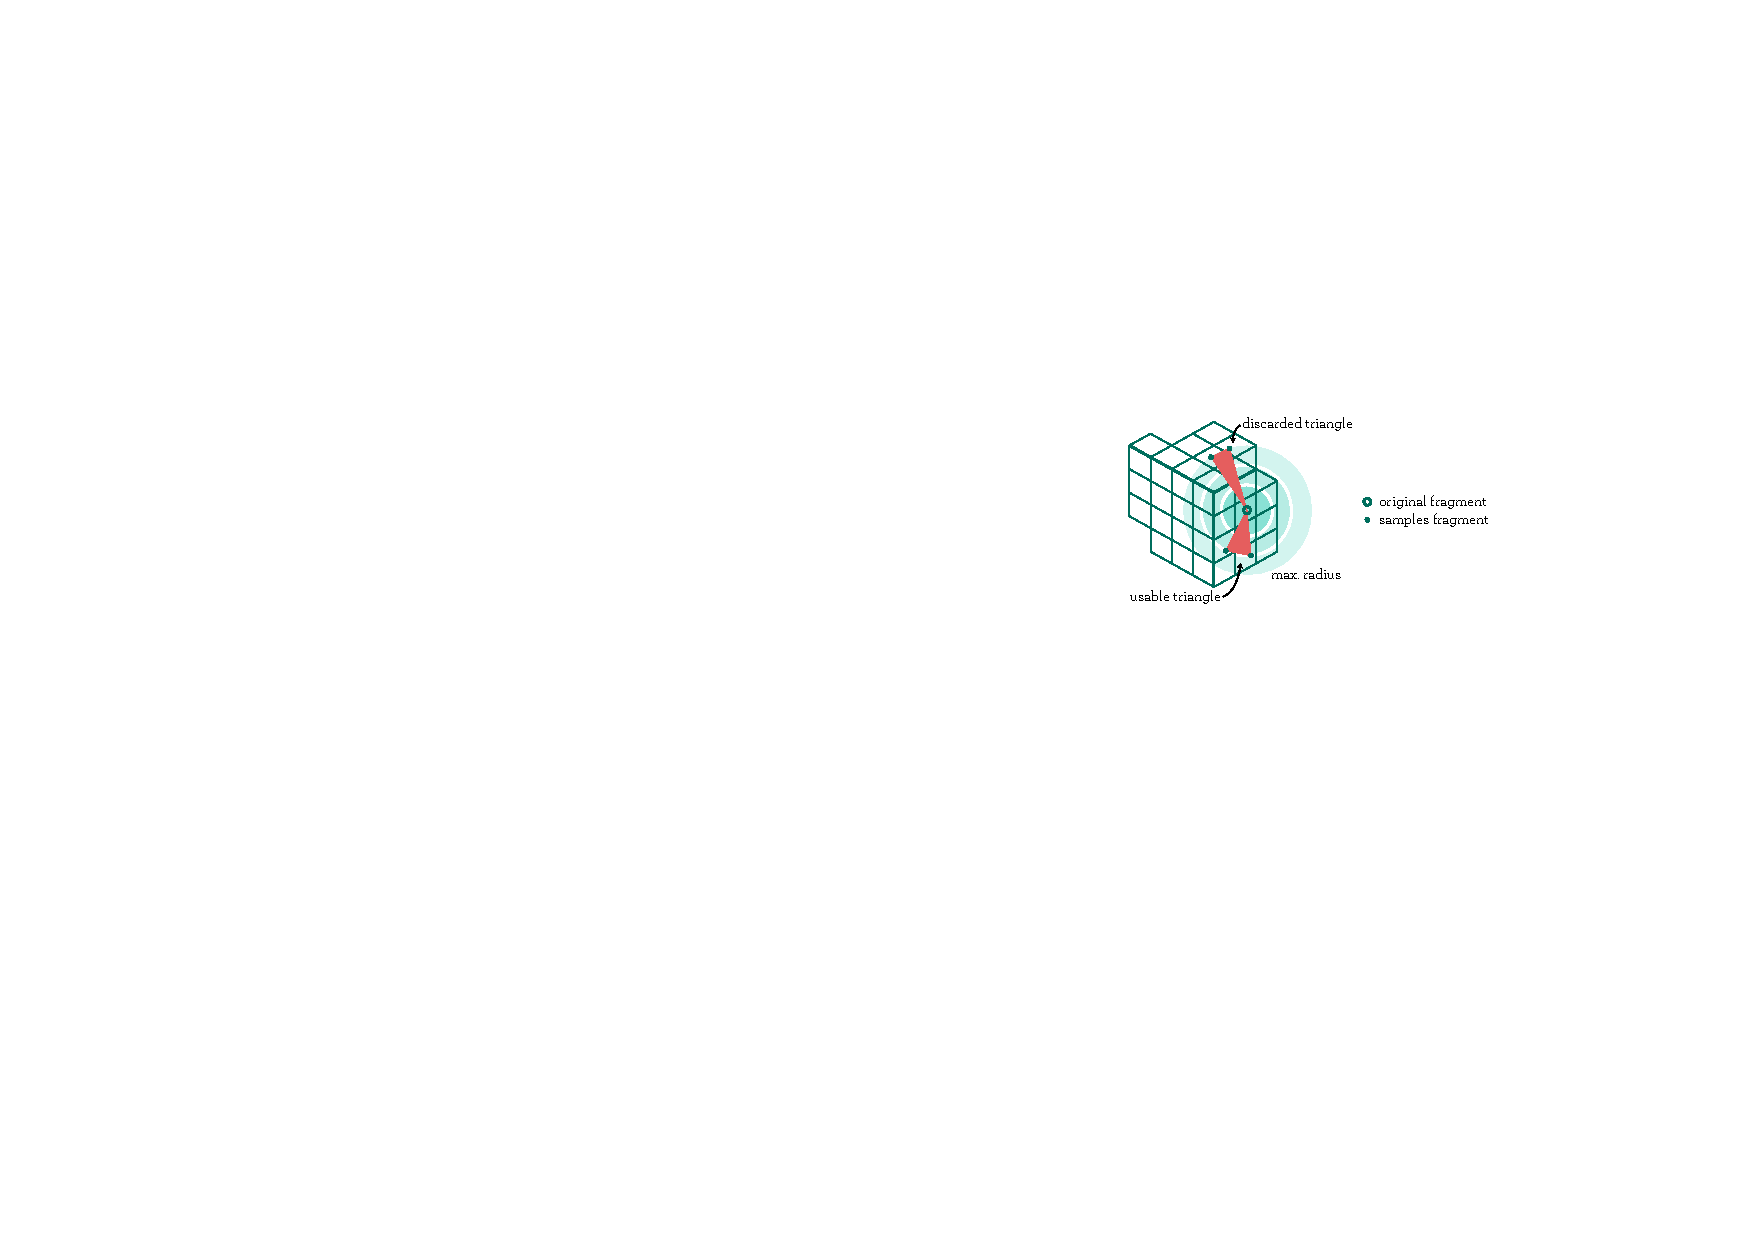
\includegraphics[scale=1.2]{figures/normal-approx.pdf}
  \caption{}
  \label{fig:normals-approx}
\end{subfigure}
\caption{Approximation of surface normals from a discontinuous depth buffer}
\label{fig:normals}
\end{figure*}